      
               
                \begin{ledgroupsized}[r]{120mm}
                \footnotesize 
                \pstart                
                \noindent\textbf{\"{U}berlieferung:}   
                \pend
                \end{ledgroupsized}
            
              
                            \begin{ledgroupsized}[r]{114mm}
                            \footnotesize 
                            \pstart \parindent -6mm
                            \makebox[6mm][l]{\textit{LiH}}Marginalien, An- und Unterstreichungen in \textsc{G. Desargues}, \cite{00034}\textit{Mani\`{e}re universelle pour pratiquer la perspective}, Paris 1648: Leibn. Marg. 175. Mehrere Unterstreichungen mit Bleistift, die nicht eindeutig Leibniz zugeordnet werden k\"{o}nnen und daher keine Ber\"{u}cksichtigung finden. \pend
                            \end{ledgroupsized}
                %\normalsize
                \vspace*{5mm}
                \begin{ledgroup}
                \footnotesize 
                \pstart
            \noindent\footnotesize{\textbf{Datierungsgr\"{u}nde}: F\"{u}r die Datierung beziehen wir uns auf die Gespr\"{a}chsnotiz N. 28. Es ist anzunehmen, dass dieser ein Gespr\"{a}ch Leibniz' mit Mariotte\protect\index{Namensregister}{\textso{Mariotte,} Edme, Seigneur de Chazeuil ca. 1620\textendash 1684} vorausging, in dem Leibniz \"{u}ber seine eigene Desargues-Lekt\"{u}re berichtete. Die Entstehungszeit der Marginalien zu Desargues d\"{u}rfte sich daher mit dem Entstehungszeitraum von N. 28 decken.}
                \pend
                \end{ledgroup}
            
                \vspace*{8mm}
                \pstart 
                \normalsize
          [Vakatseite: \textit{Notiz von Leibniz}] Figure fautive p. 86. de la perspective  cette methode n'est pas ass\'{e}s propre \`{a} eclairer l'esprit, parce qu'elle ne nous fait connoistre qu'\`{a} la fin les raisons pourquoy l'auteur nous mene comme cela. Elle n'est pas \edtext{si}{\lemma{}\Afootnote{si \textit{ erg.} \textit{ L}}} propre \`{a} l'invention mais elle a l'avantage de surprendre les lecteurs, quand ils se trouuent men\'{e}s \`{a} quelque chose sans y penser; et on retient mieux les choses qu'on admire. V. p. 57. 58. p. 83. fin. p. 84 fin.\pend \pstart  Dans la page 28 on ne voit pas bien \edtext{encore}{\lemma{}\Afootnote{encore \textit{ erg.} \textit{ L}}} la raison, pourquoy \textit{CZ} et \textit{EL} doiuent estre prises telles qu'il dit.\pend \pstart J'ay adjout\'{e} quelque chose, (marqu\'{e} de NB) p. 86.\pend
          \pstart \hspace{2mm} [p.~37] Sur quoy vous pouuez iuger qu'il en est de mesme de toute autre chose que du corps humain, et que quand vous aurez apris les regles de la perspectiue, pour faire le pourtraict de quelque chose que ce puisse estre sur le deuis que vous aurez des mesures necessaires \`{a} cela, vous ne serez non plus oblig\'{e} de vous y seruir, si vous ne voulez, de la regle, et du compas: Mais vous le pourrez faire, si bon vous semble, ainsi que celuy du corps humain, sous la conduite de l'imagination, et de l'oeil\footnote{\textit{Leibniz unterstreicht}: quand [...] l'oeil}, auec la connoissance que vous aurez des mesures de ses parties; [...].\pend
          \pstart [p.~45] De plus il faut imaginer, qu'vne surface plate\footnote{\textit{Leibniz unterstreicht}: plate} et transparante, encore immobile en vne place, trauerse toute l'estendu\"{e} ou epesseur du rayonnement sous lequel l'oeil\protect\index{Sachverzeichnis}{oeil} void le sujet sans en interrompre aucunes de lignes [...].\pend \pstart  La surface plate\footnote{\textit{Leibniz unterstreicht}: plate} qu'on entend qui trauerse le rayonnement de la veu\"{e} est nomm\'{e}e par quelques vns la \textit{transparance} par d'autres le verre\protect\index{Sachverzeichnis}{verre}, la \textit{section}, et par d'autres d'vn autre nom.\pend
          \pstart [p.~55] Quand le plan du tableau se trouue paralelle \`{a} la figure\footnote{\textit{Leibniz unterstreicht}: Quand [...] figure} qui est le suiet, lors en quelle part que l'oeil\protect\index{Sachverzeichnis}{oeil} se trouue situ\'{e}, la figure de representation est to\^{u}jours entierement de mesme forme que celle du suiet: et de plus vne mesme grandeur sert \`{a} la mesurer toute en tout sens d'vn bout \`{a} l'autre.\\Quand l'oeil\protect\index{Sachverzeichnis}{oeil} est entendu situ\'{e} \`{a} distance infinie\footnote{\textit{Leibniz unterstreicht}: Quand [...] infinie}, ou intermin\'{e}e, en quelque sorte que le plan du tableau soit situ\'{e}, la figure de representation est de telle espece, que ces deux choses s'y trouuent; [...].\pend
\protect\clearpage
\begin{center}
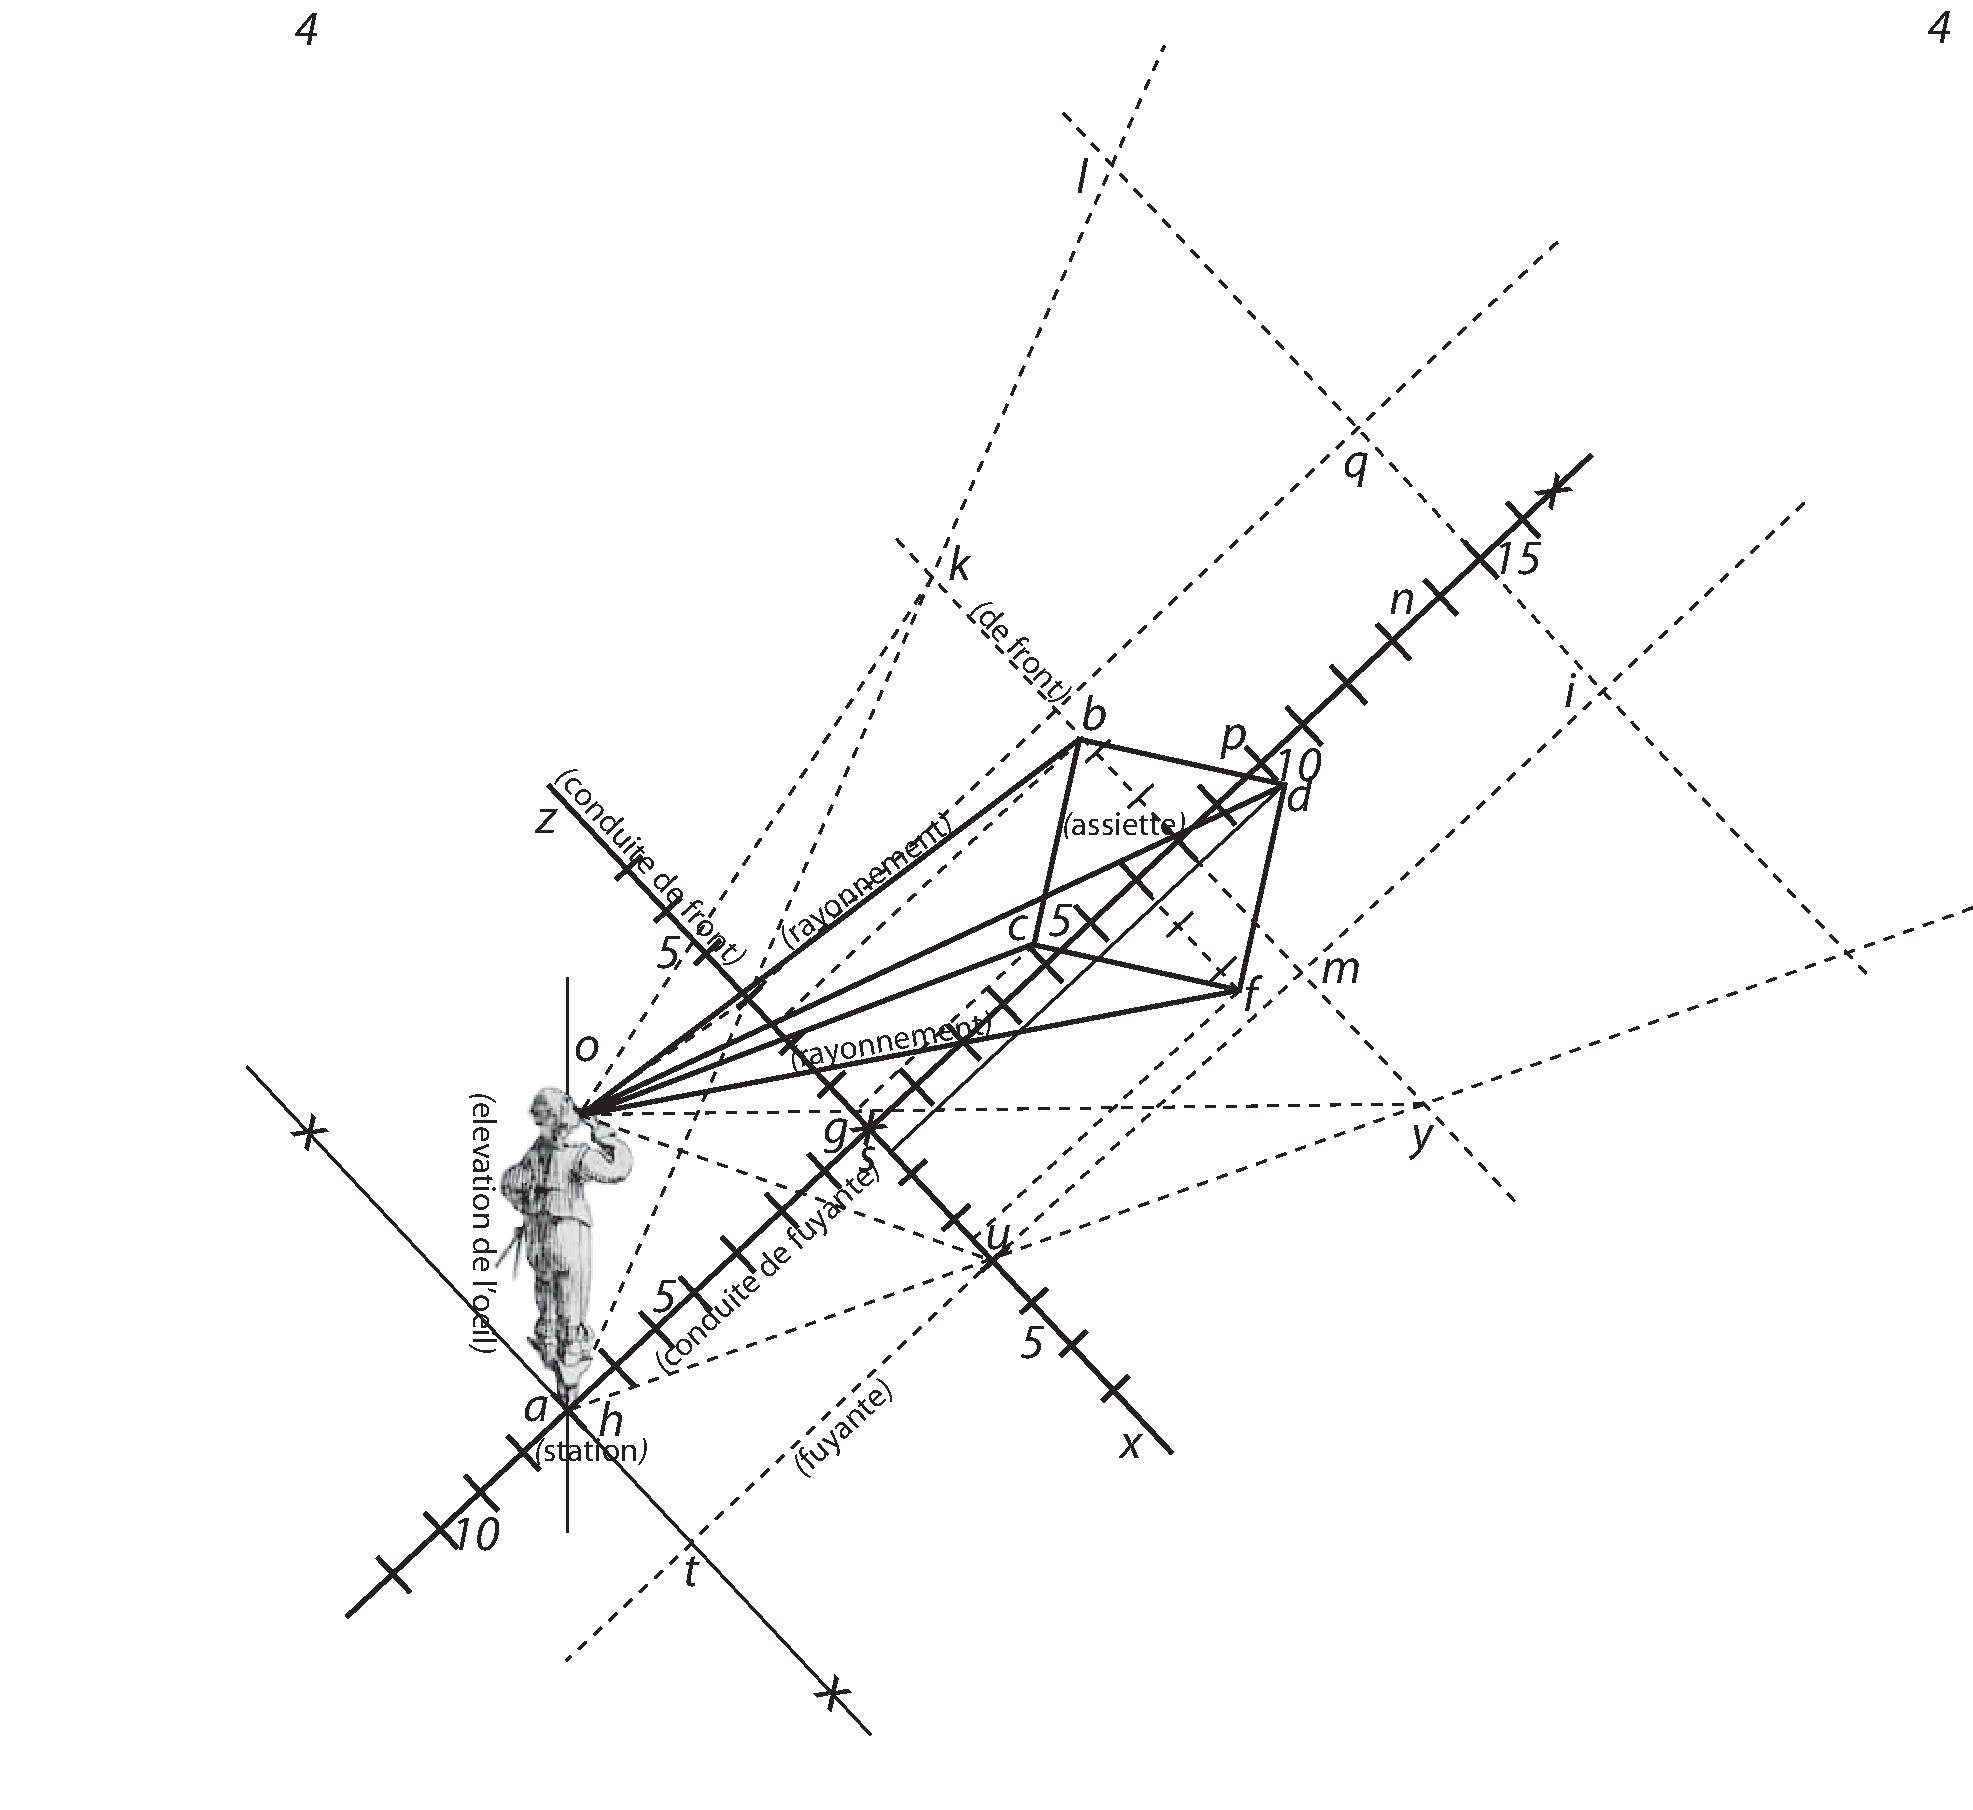
\includegraphics[width=1.0\textwidth]{images/T4-Desargues}
\\\rule[-4mm]{0mm}{10mm}\textit{[Fig. 1]}
\protect\clearpage
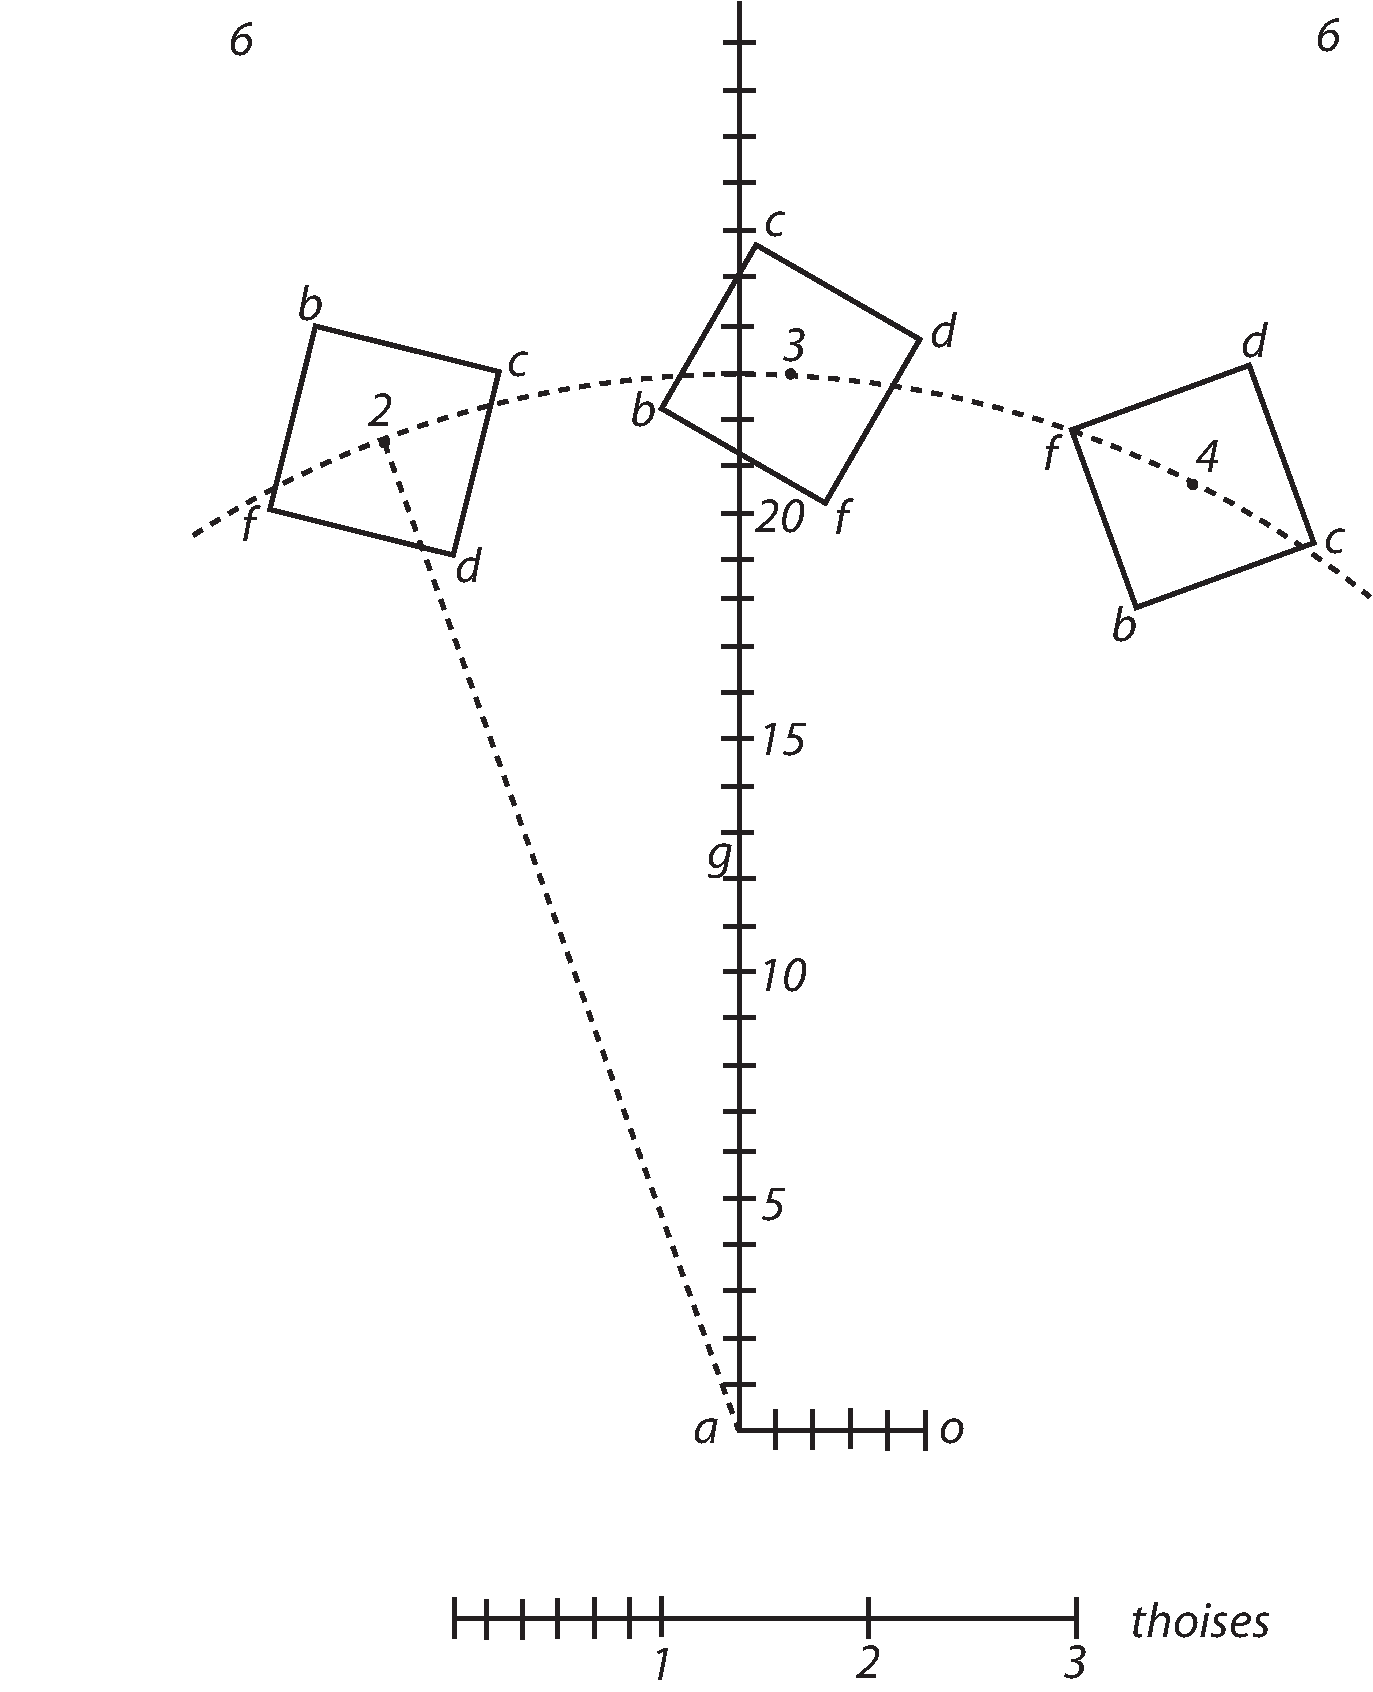
\includegraphics[width=0.7\textwidth]{images/T6-Desargues}\end{center}
\protect\rule[0mm]{60mm}{0mm}\textit{[Fig. 2]}
\footnote{\textit{Im mittleren Teil der Zeichnung links}: la 4\textsuperscript{me} planche commence les nombres par \textit{g}}
\protect\clearpage\begin{center}
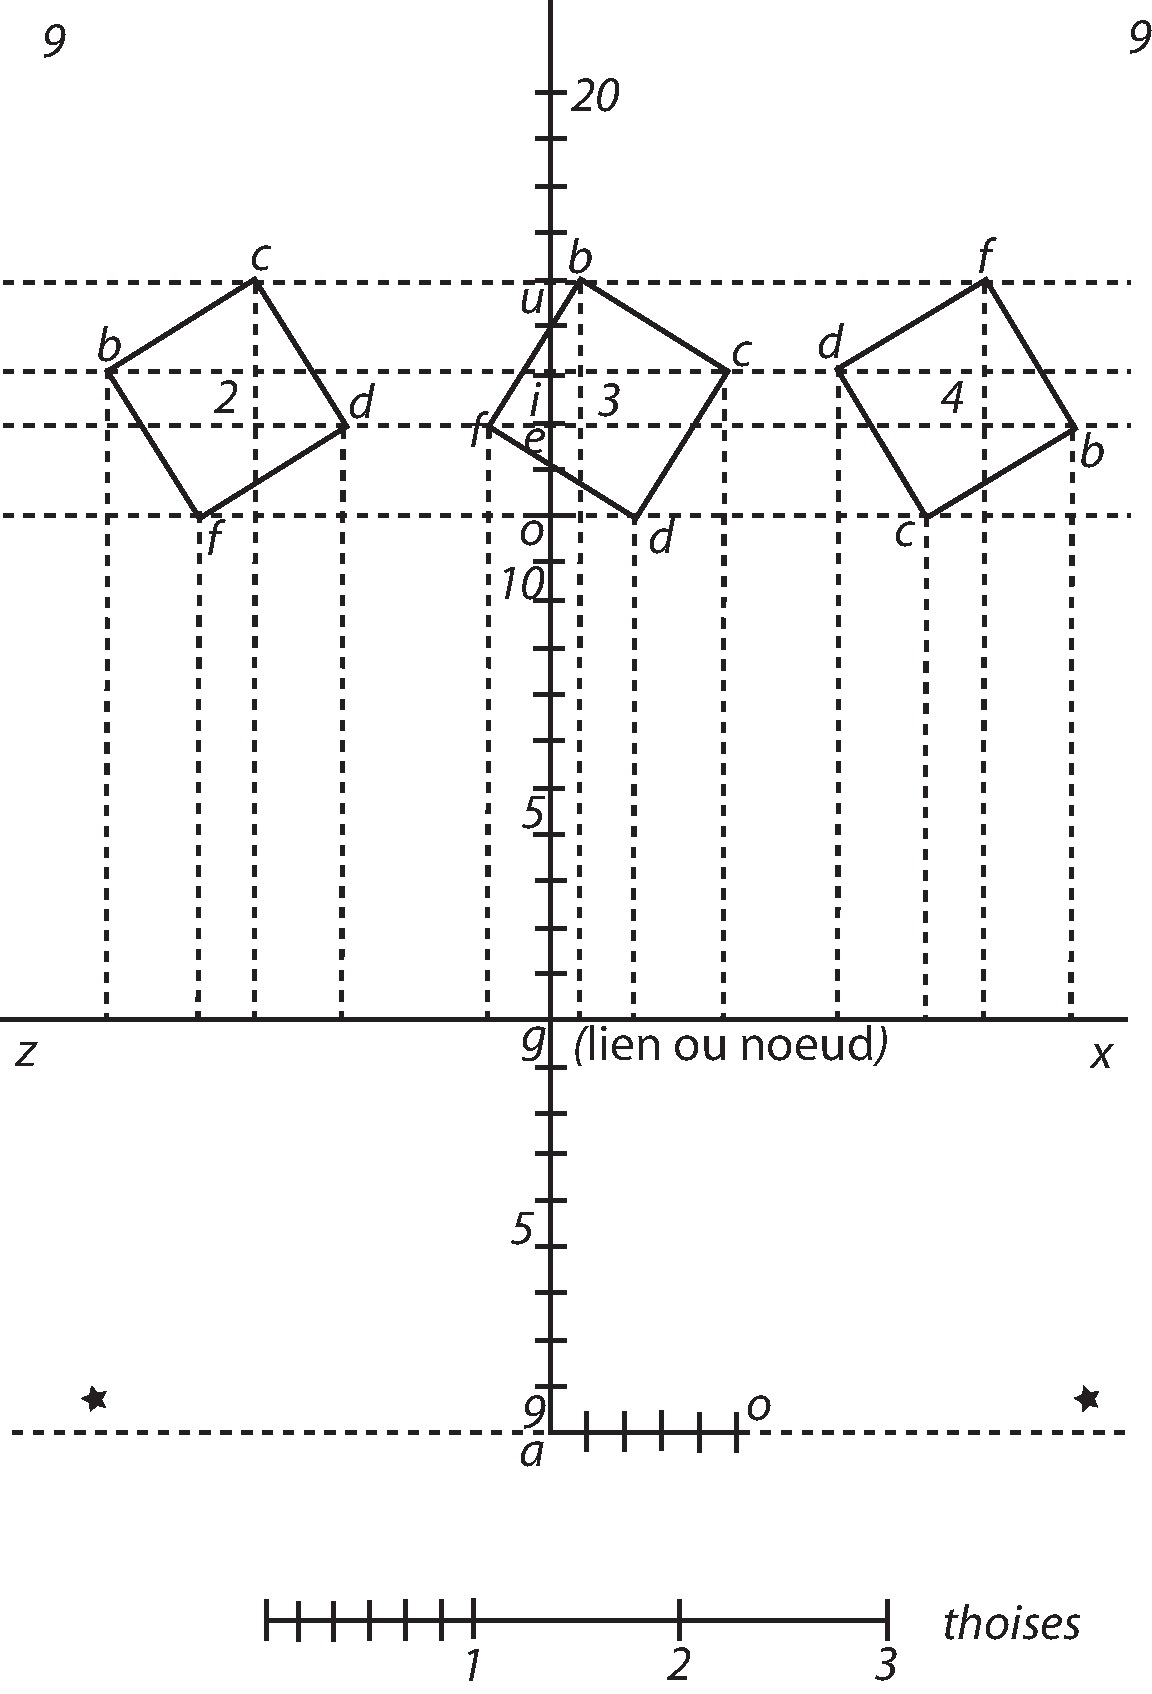
\includegraphics[width=0.7\textwidth]{images/T9-Desargues}
\\\textit{[Fig. 3]}
\protect\clearpage
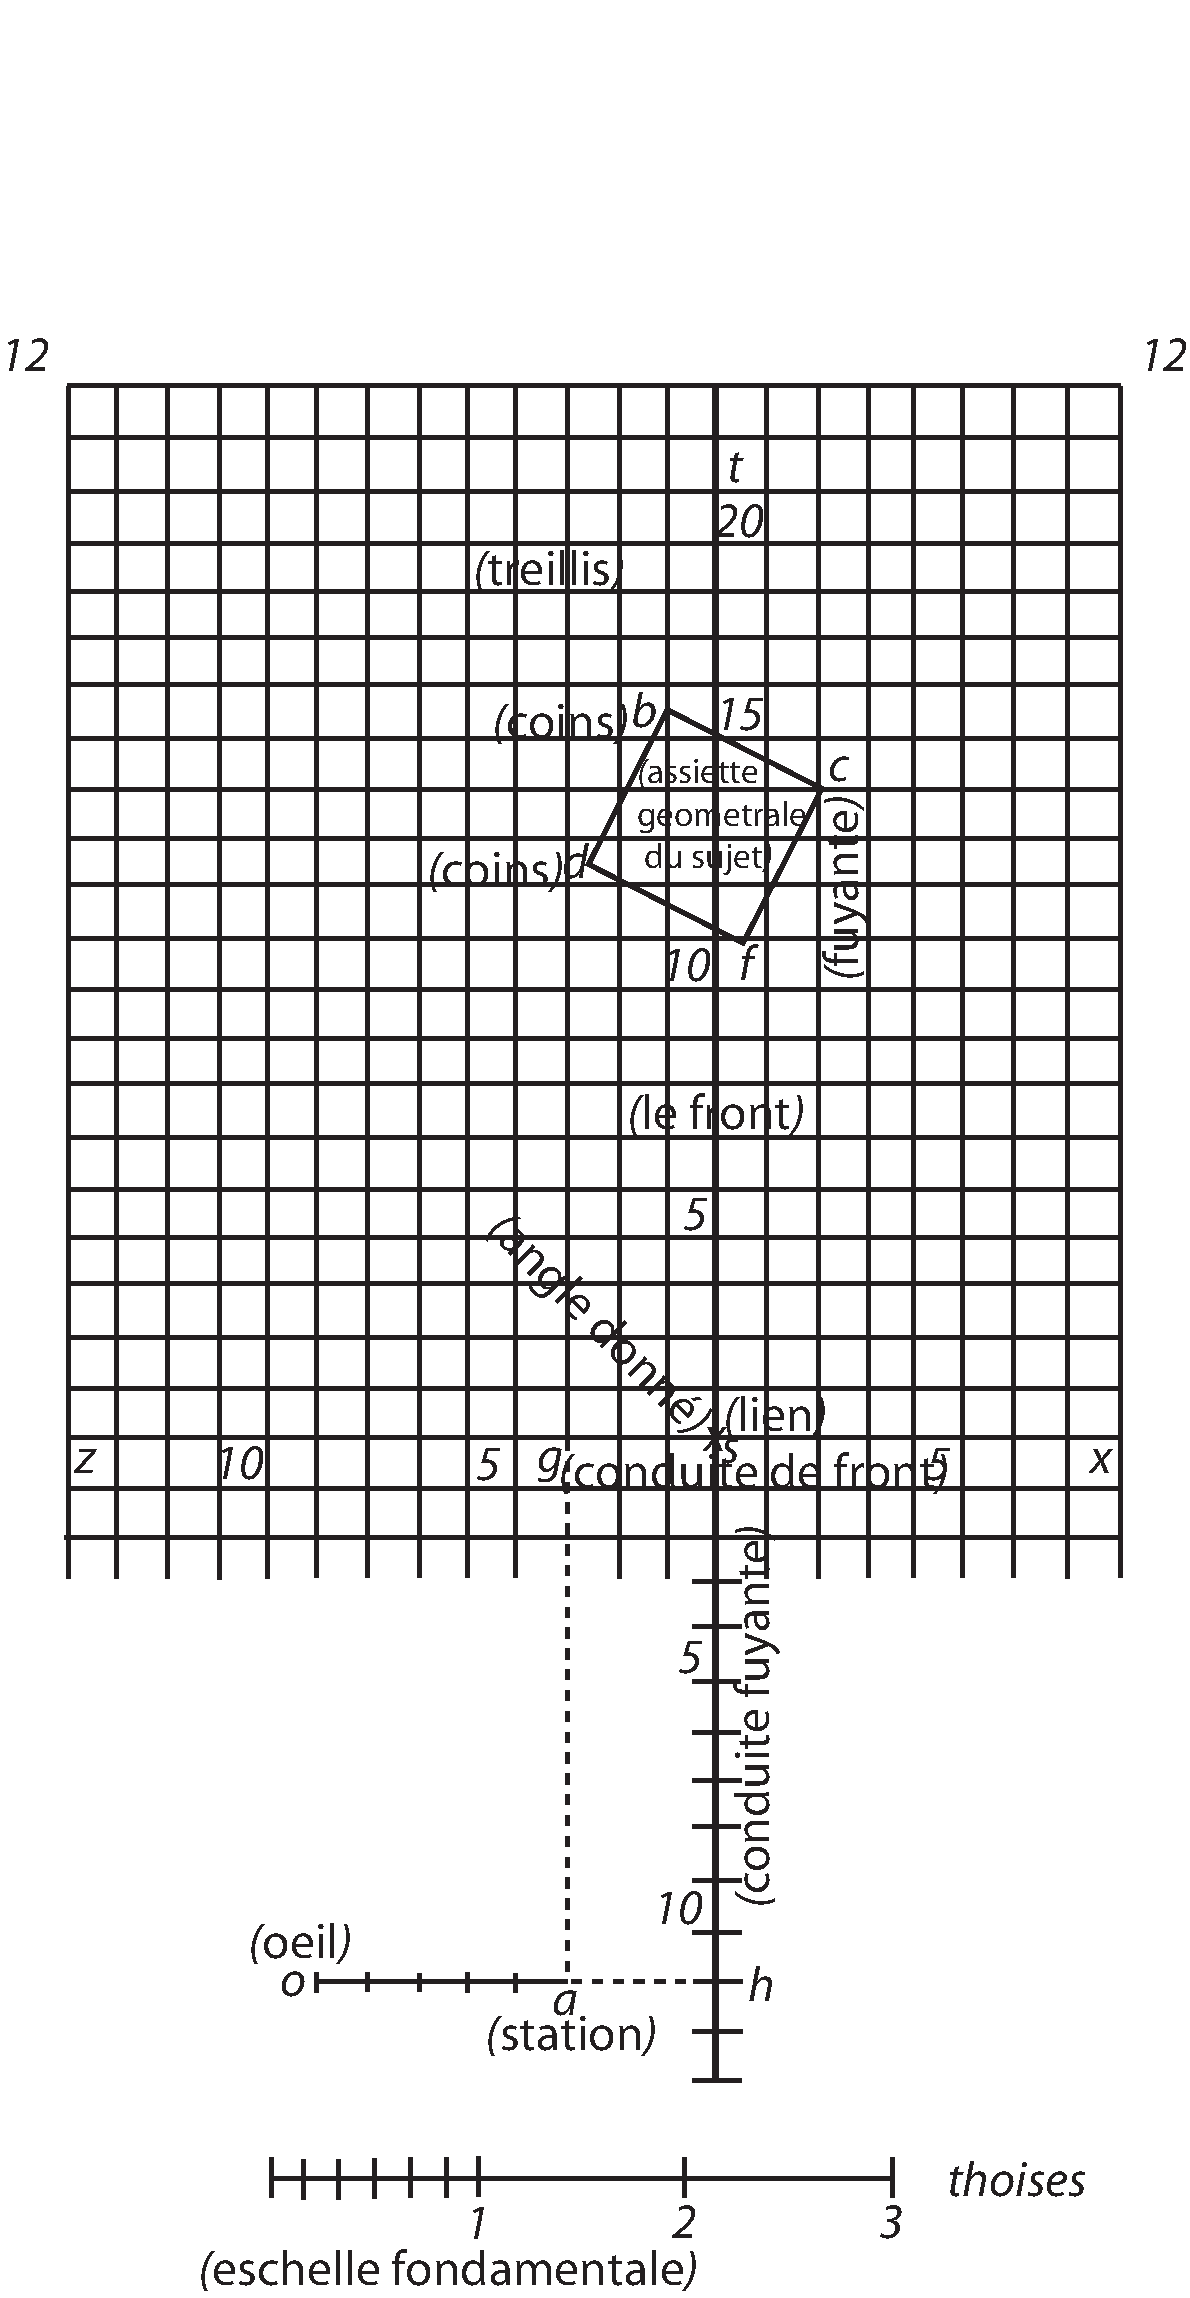
\includegraphics[width=0.7\textwidth]{images/T12-Desargues}
\\\textit{[Fig. 4]}
\protect\clearpage
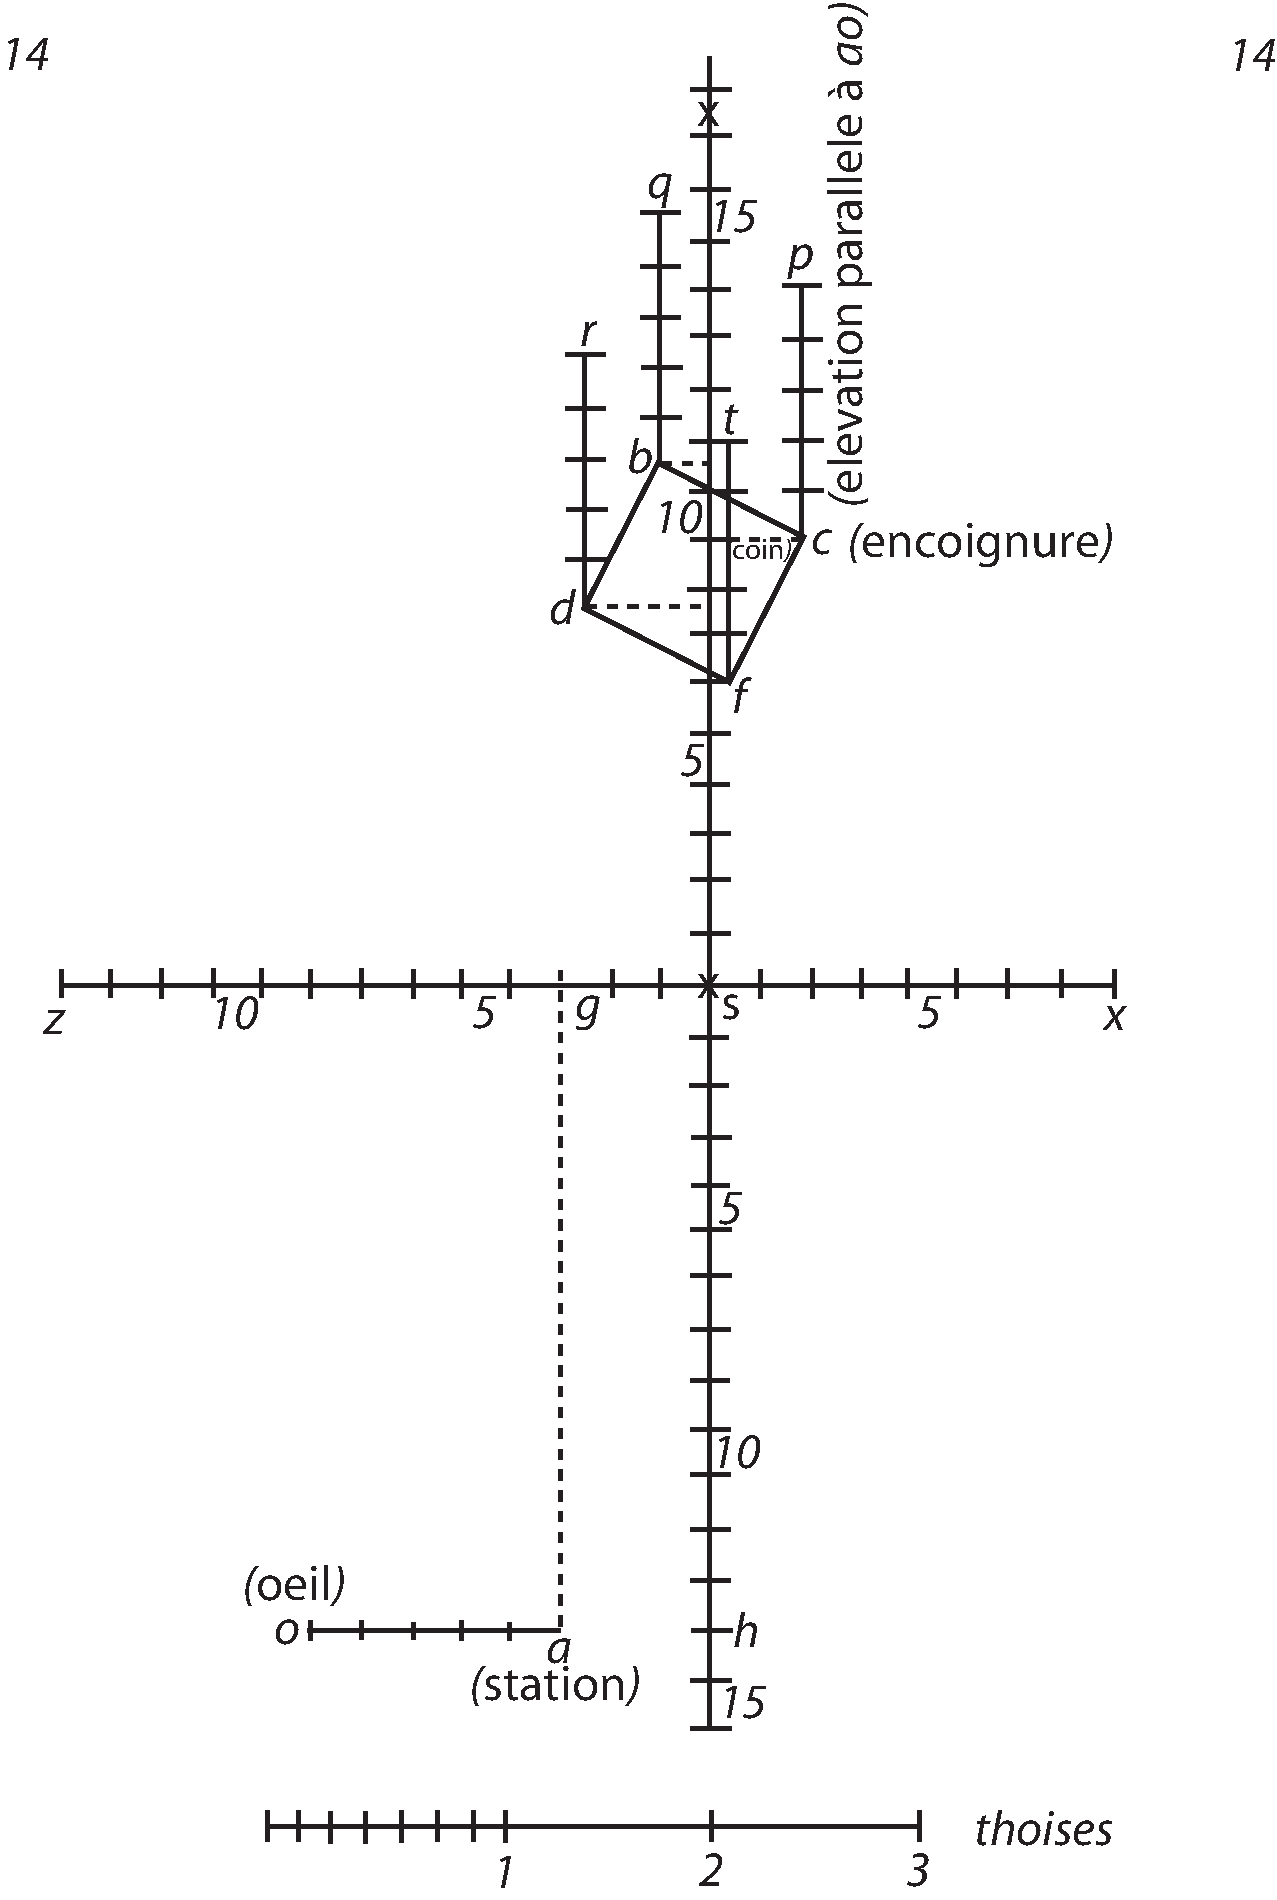
\includegraphics[width=0.78\textwidth]{images/T14-Desargues}
\\\rule[-4mm]{0mm}{10mm}\textit{[Fig. 5]}
\protect\clearpage
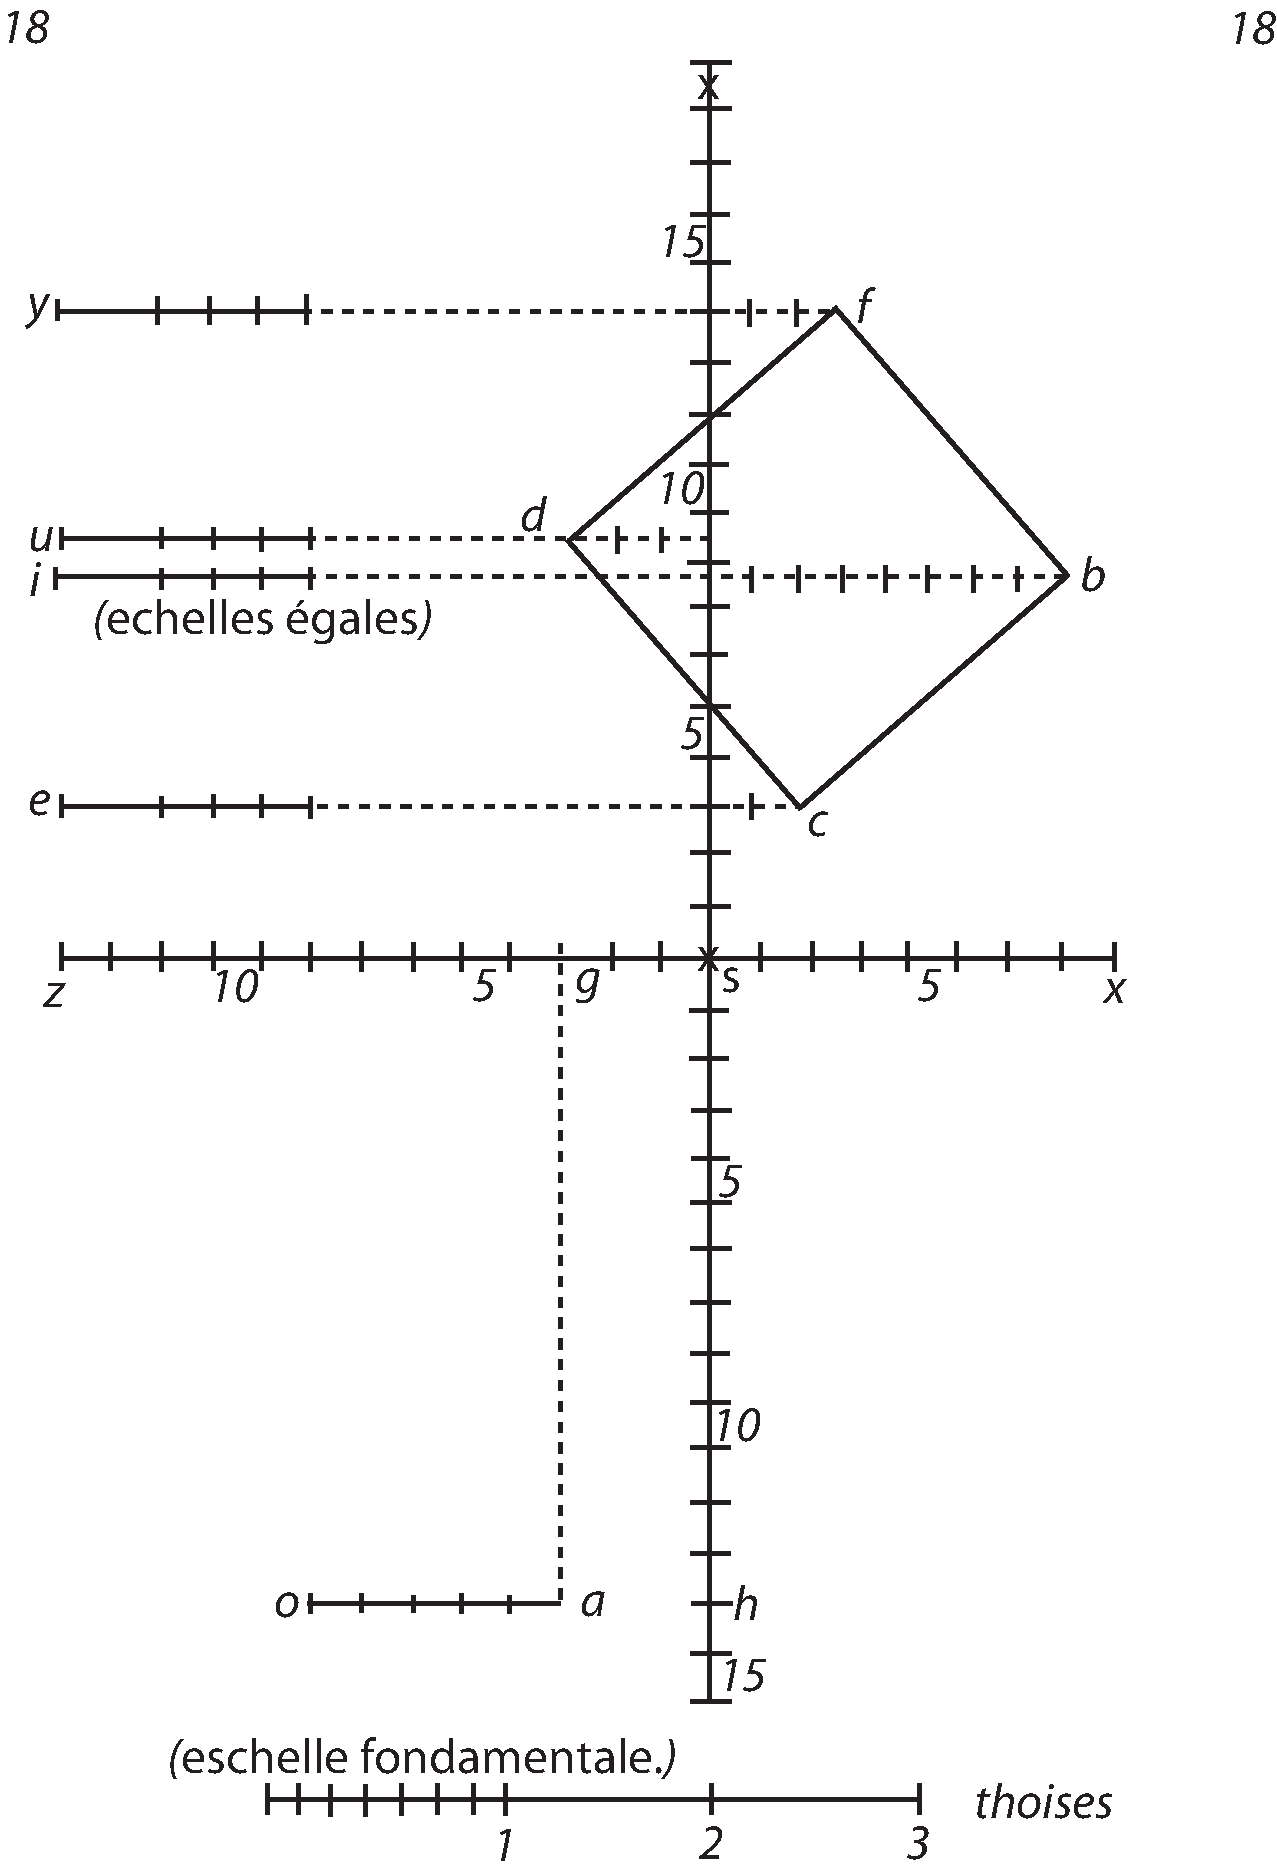
\includegraphics[width=0.7\textwidth]{images/T18-Desargues}
\\\rule[-4mm]{0mm}{10mm}\textit{[Fig. 6]}
\protect\clearpage
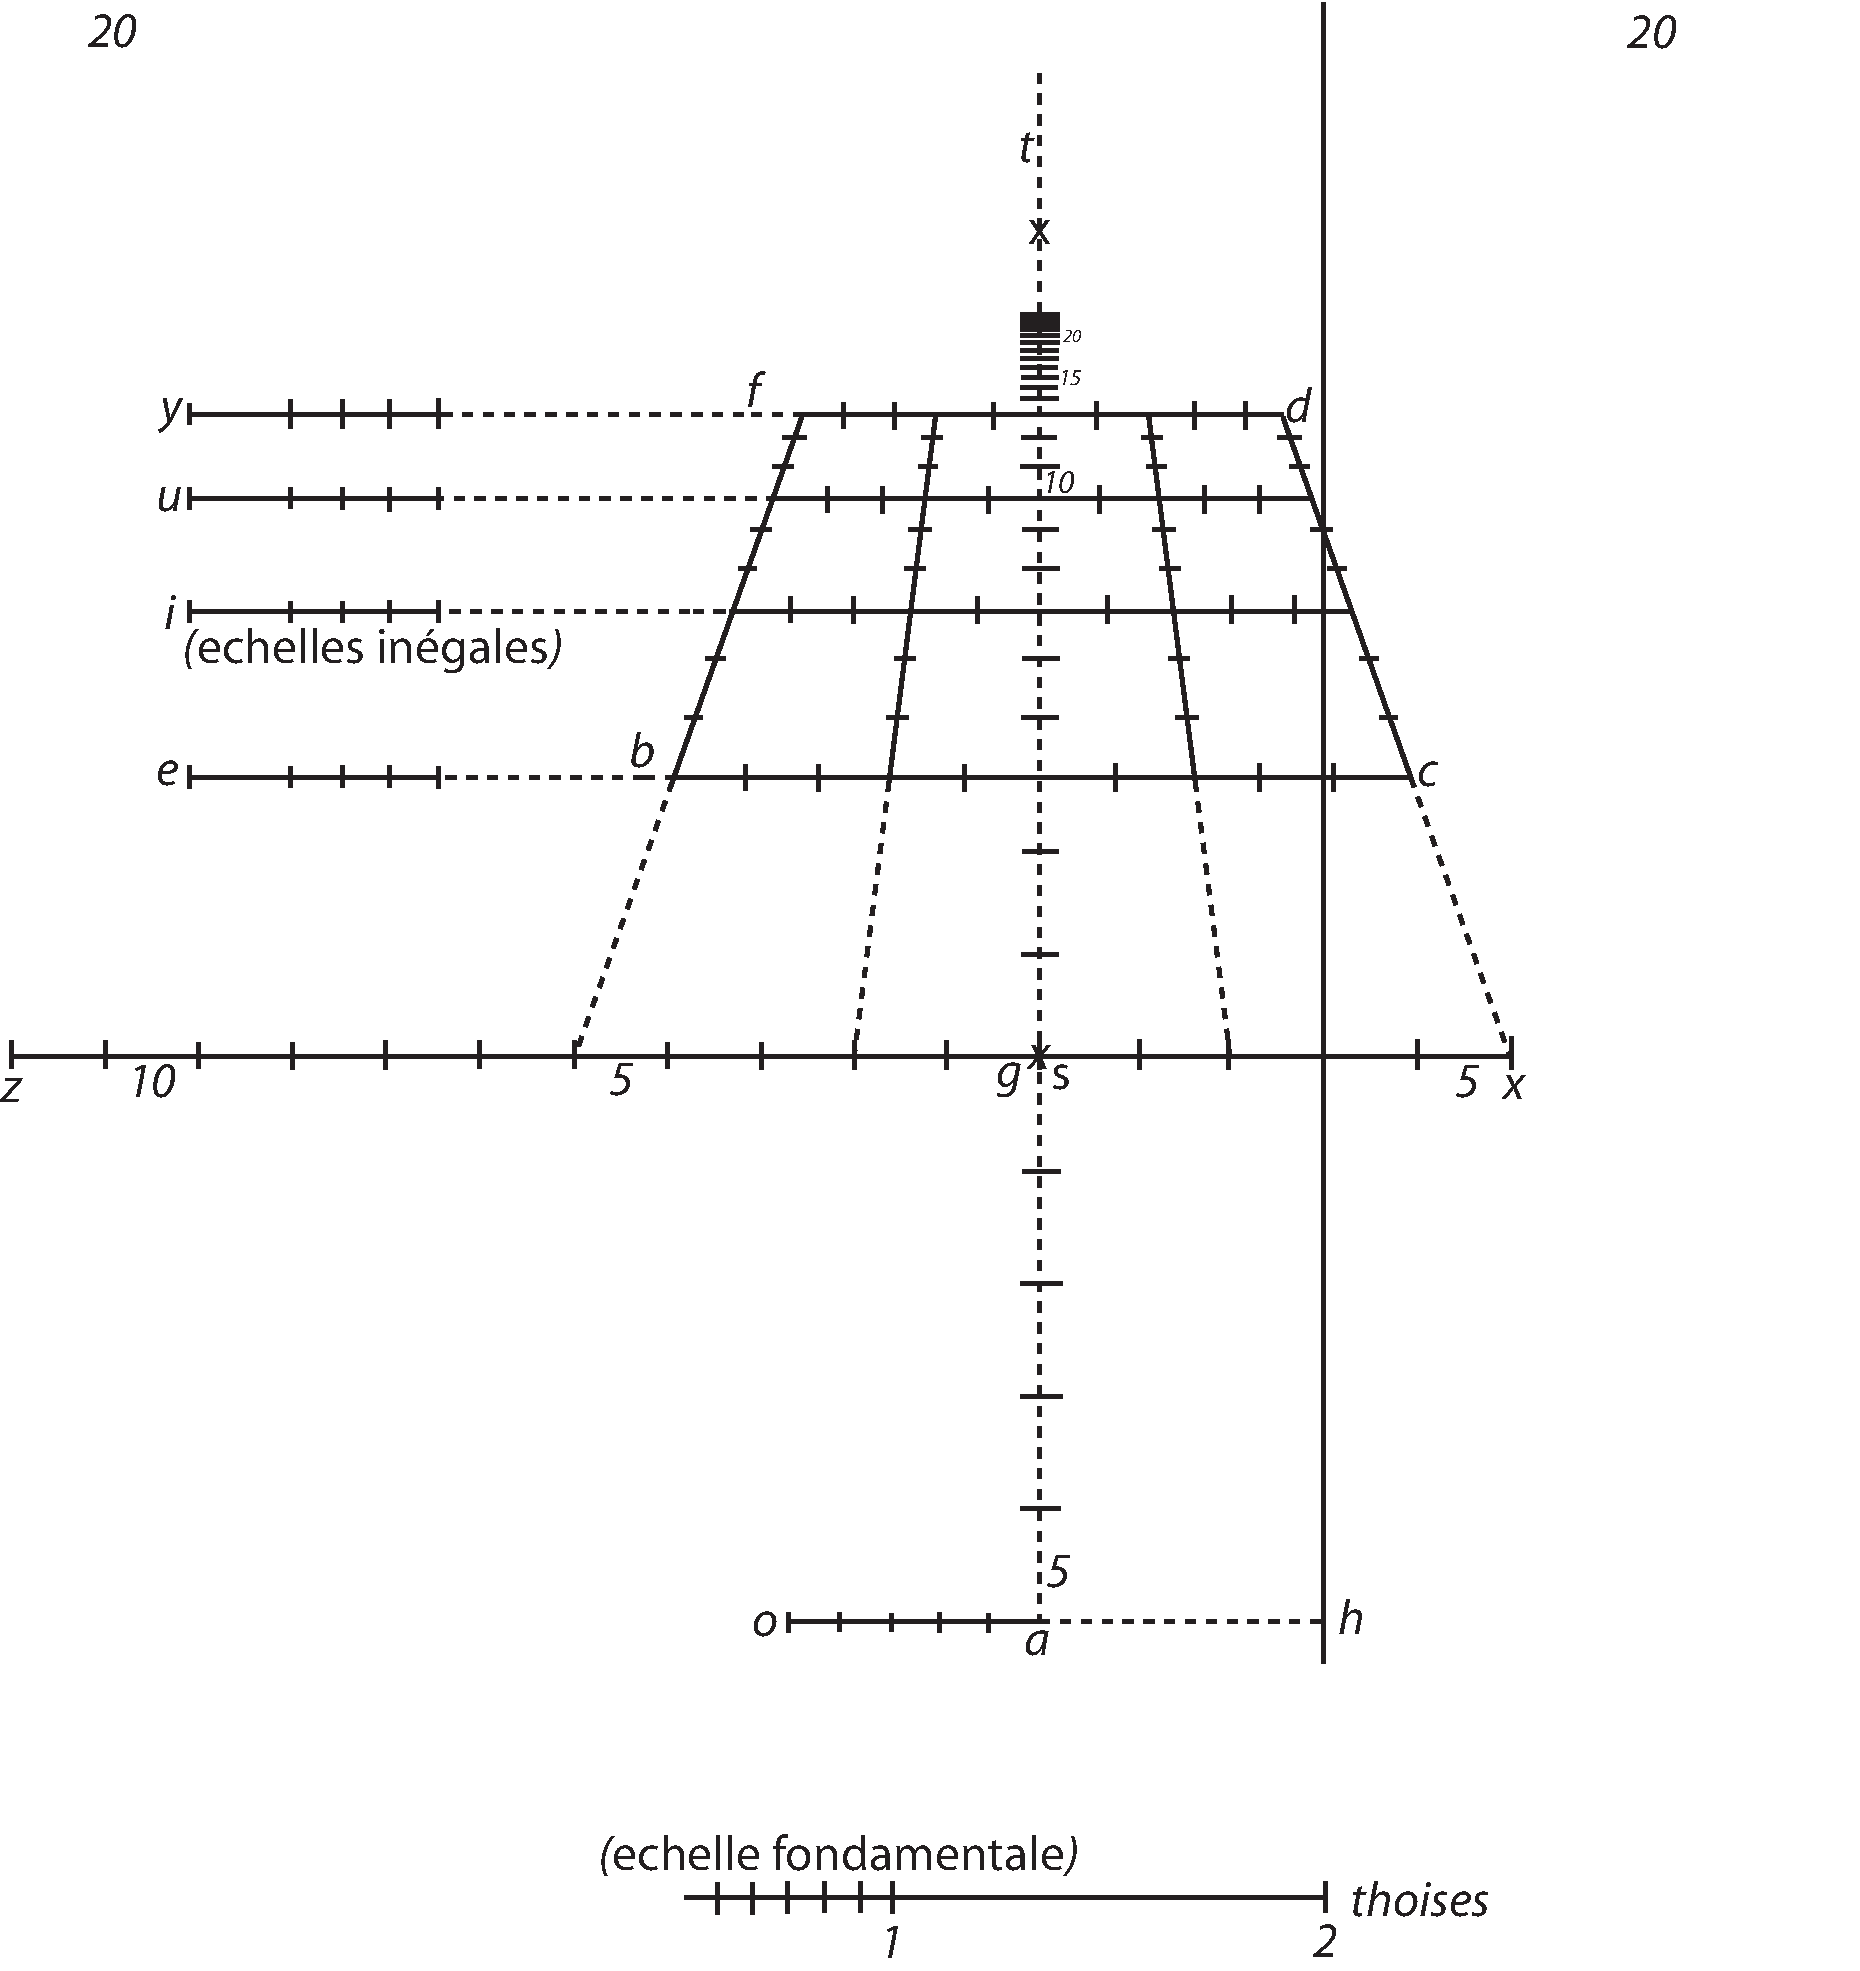
\includegraphics[width=0.9\textwidth]{images/T20-Desargues}
\\\rule[-4mm]{0mm}{10mm}\textit{[Fig. 7]}
\protect\clearpage
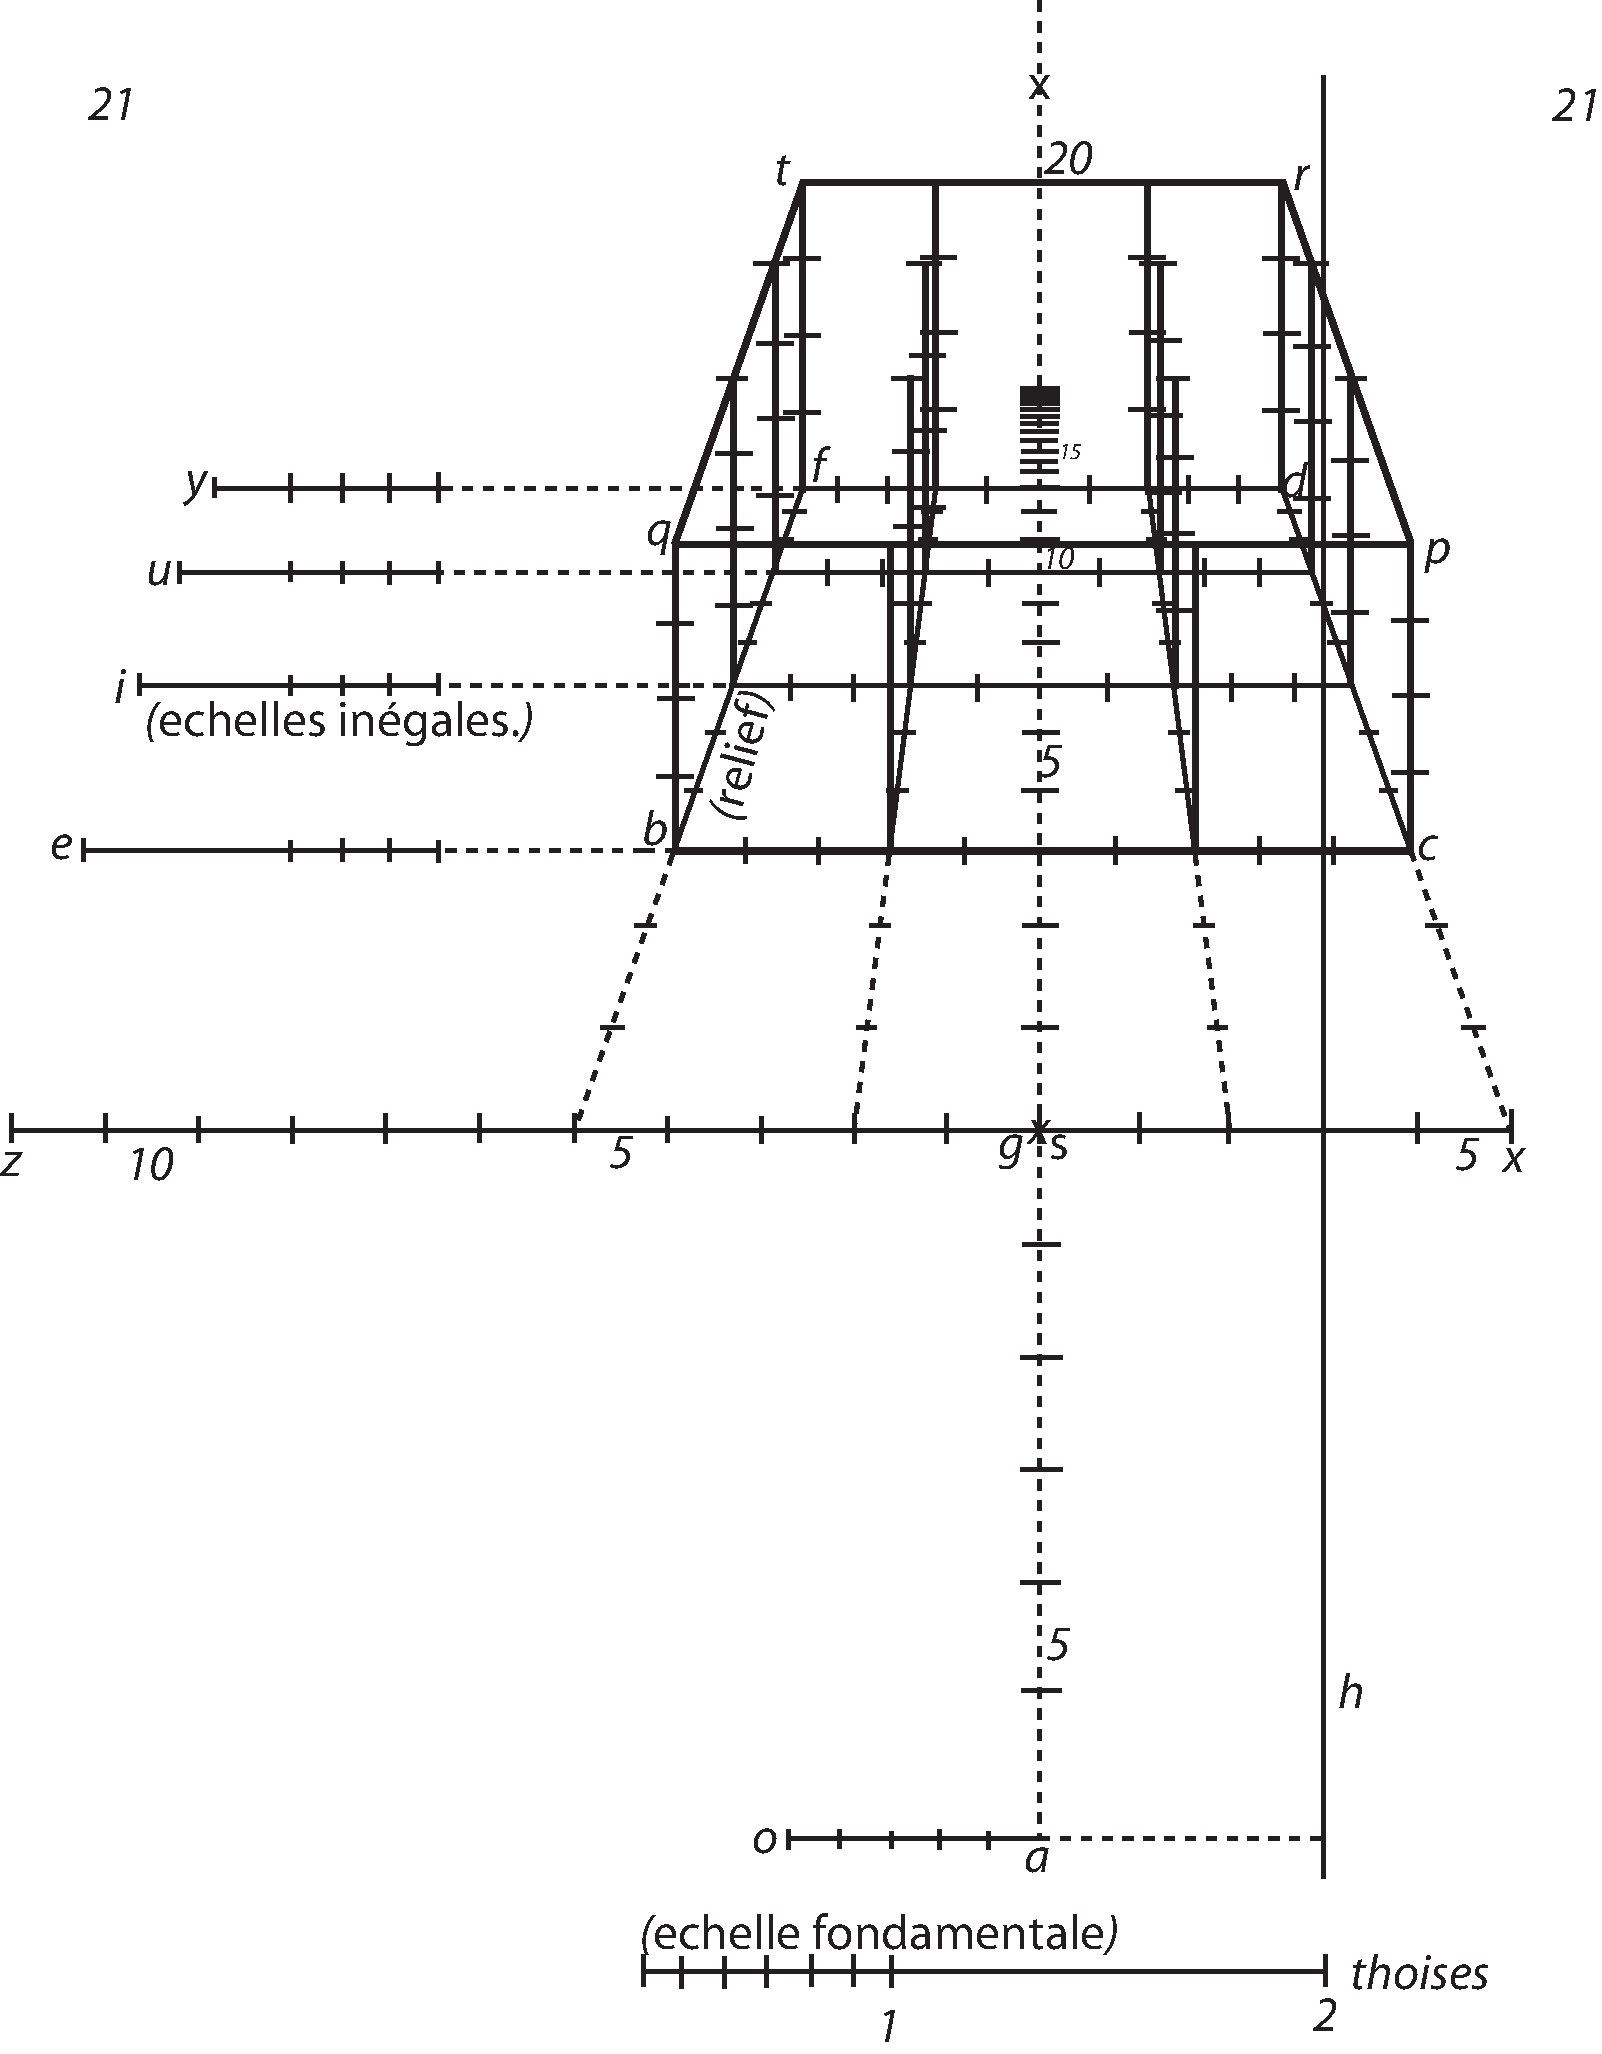
\includegraphics[width=0.9\textwidth]{images/T21-Desargues}
\\\rule[-4mm]{0mm}{10mm}\textit{[Fig. 8]}
\protect\clearpage
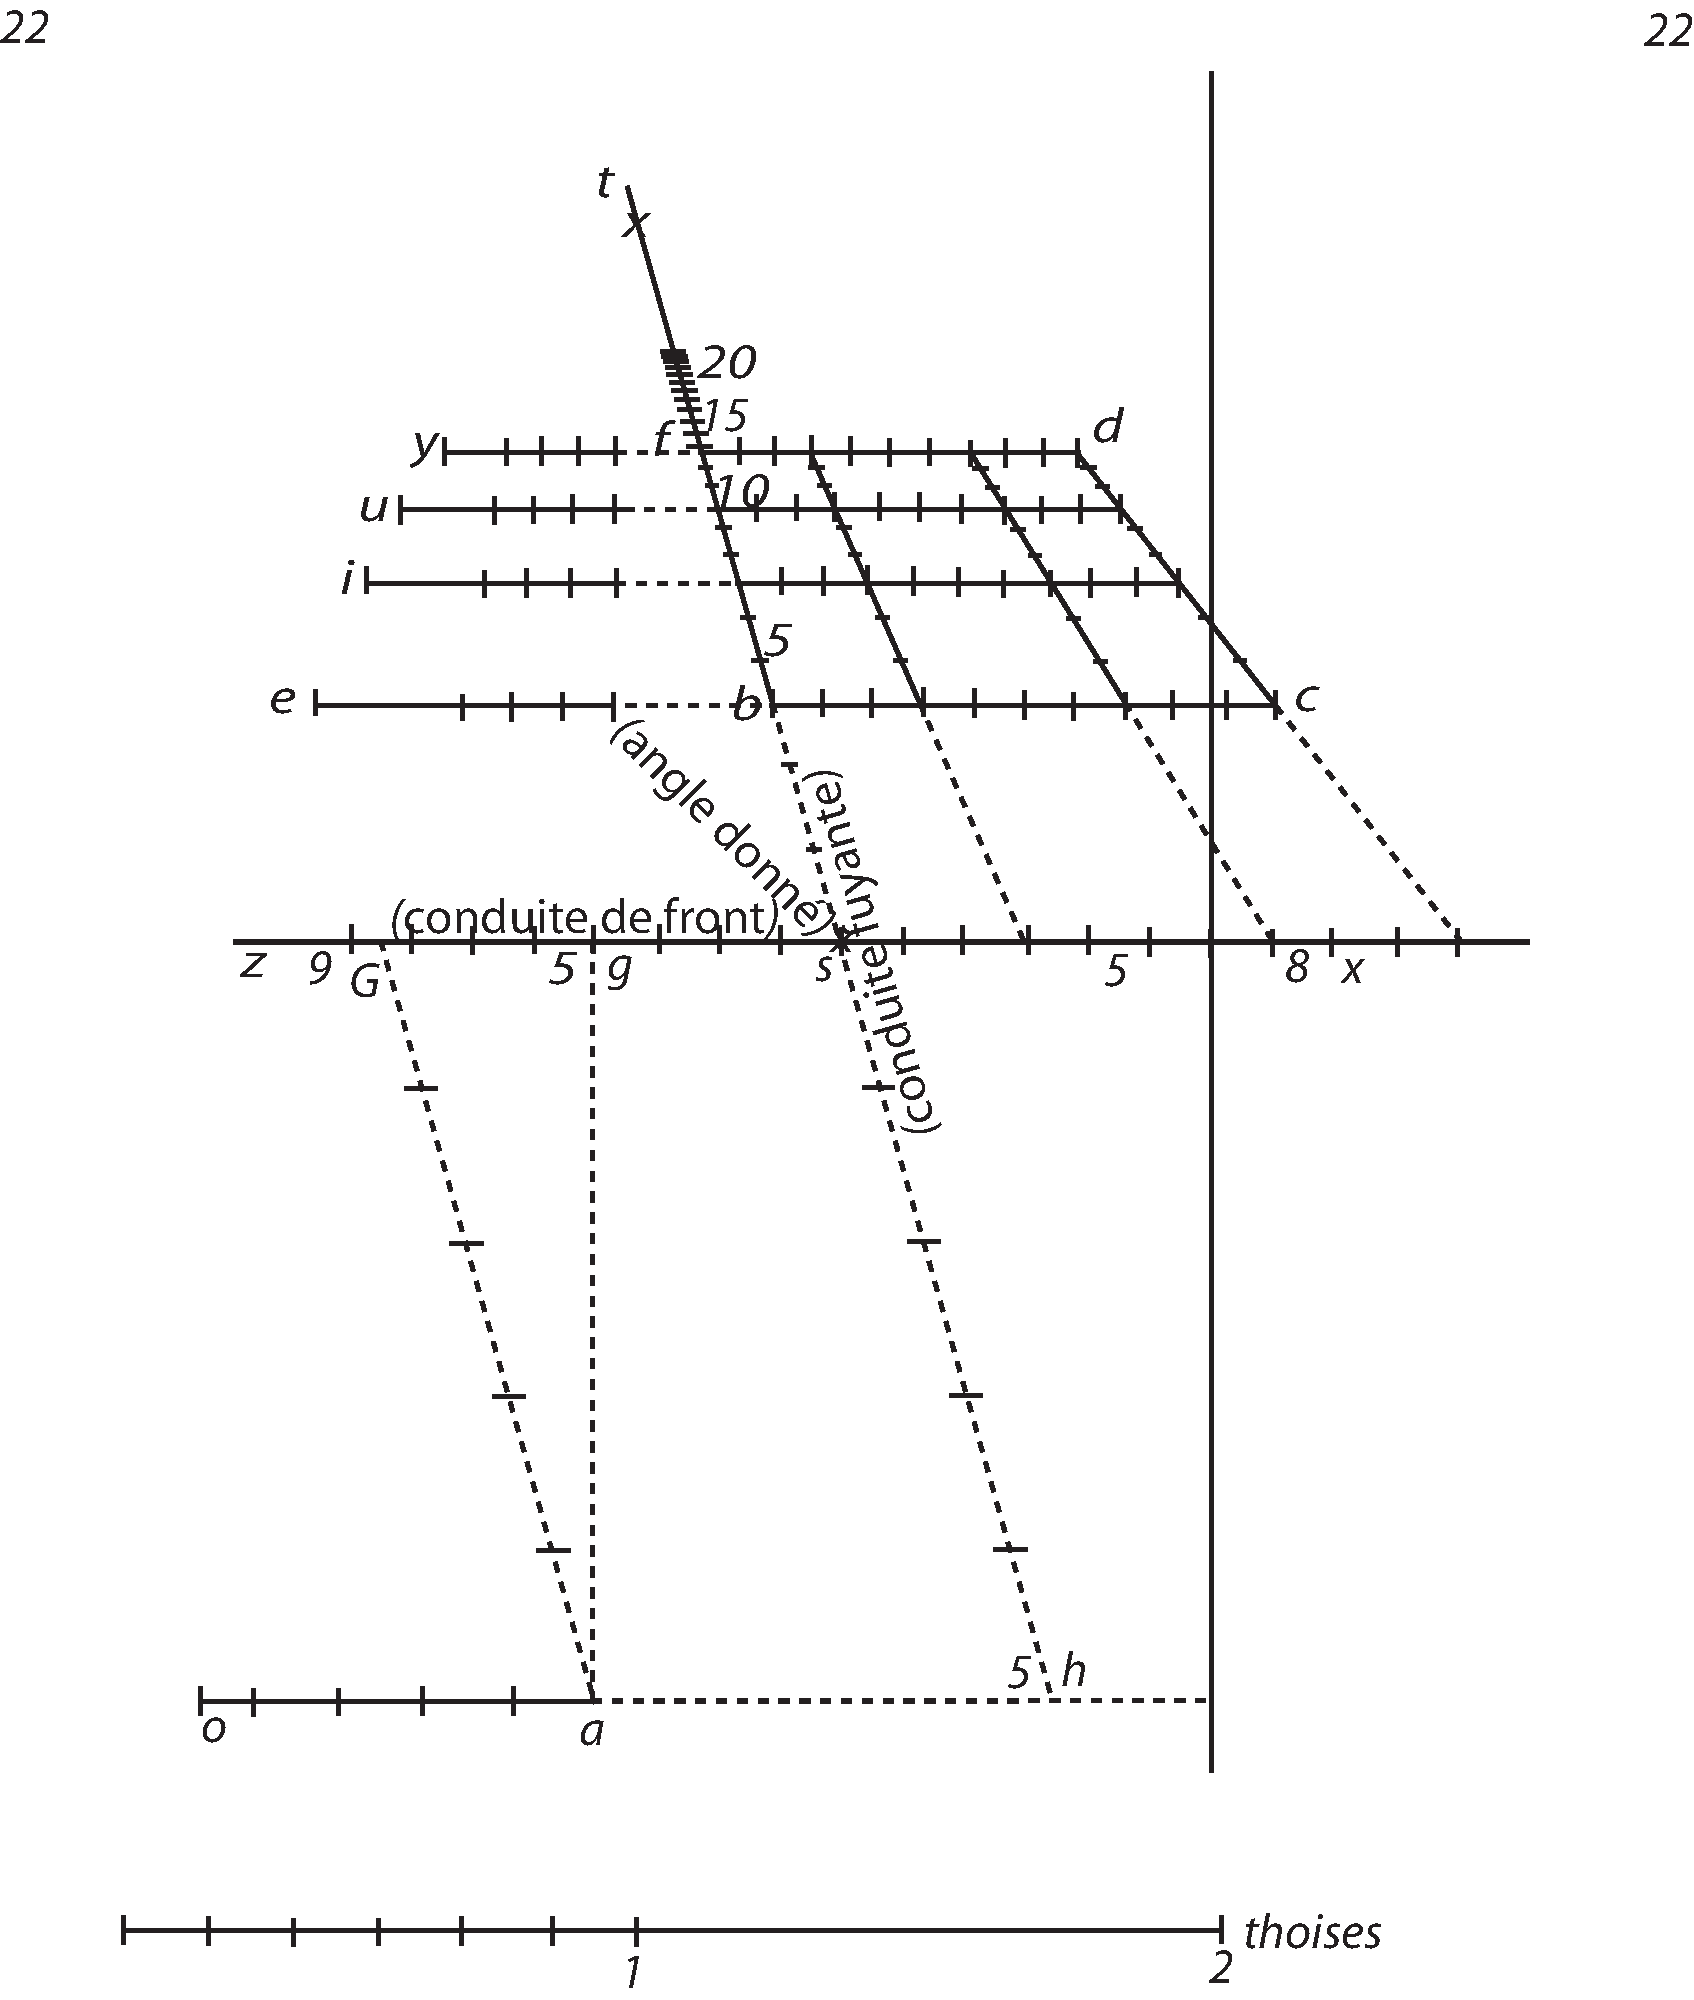
\includegraphics[width=1.0\textwidth]{images/T22-Desargues}
\\\rule[-4mm]{0mm}{10mm}\textit{[Fig. 9]}
\protect\clearpage
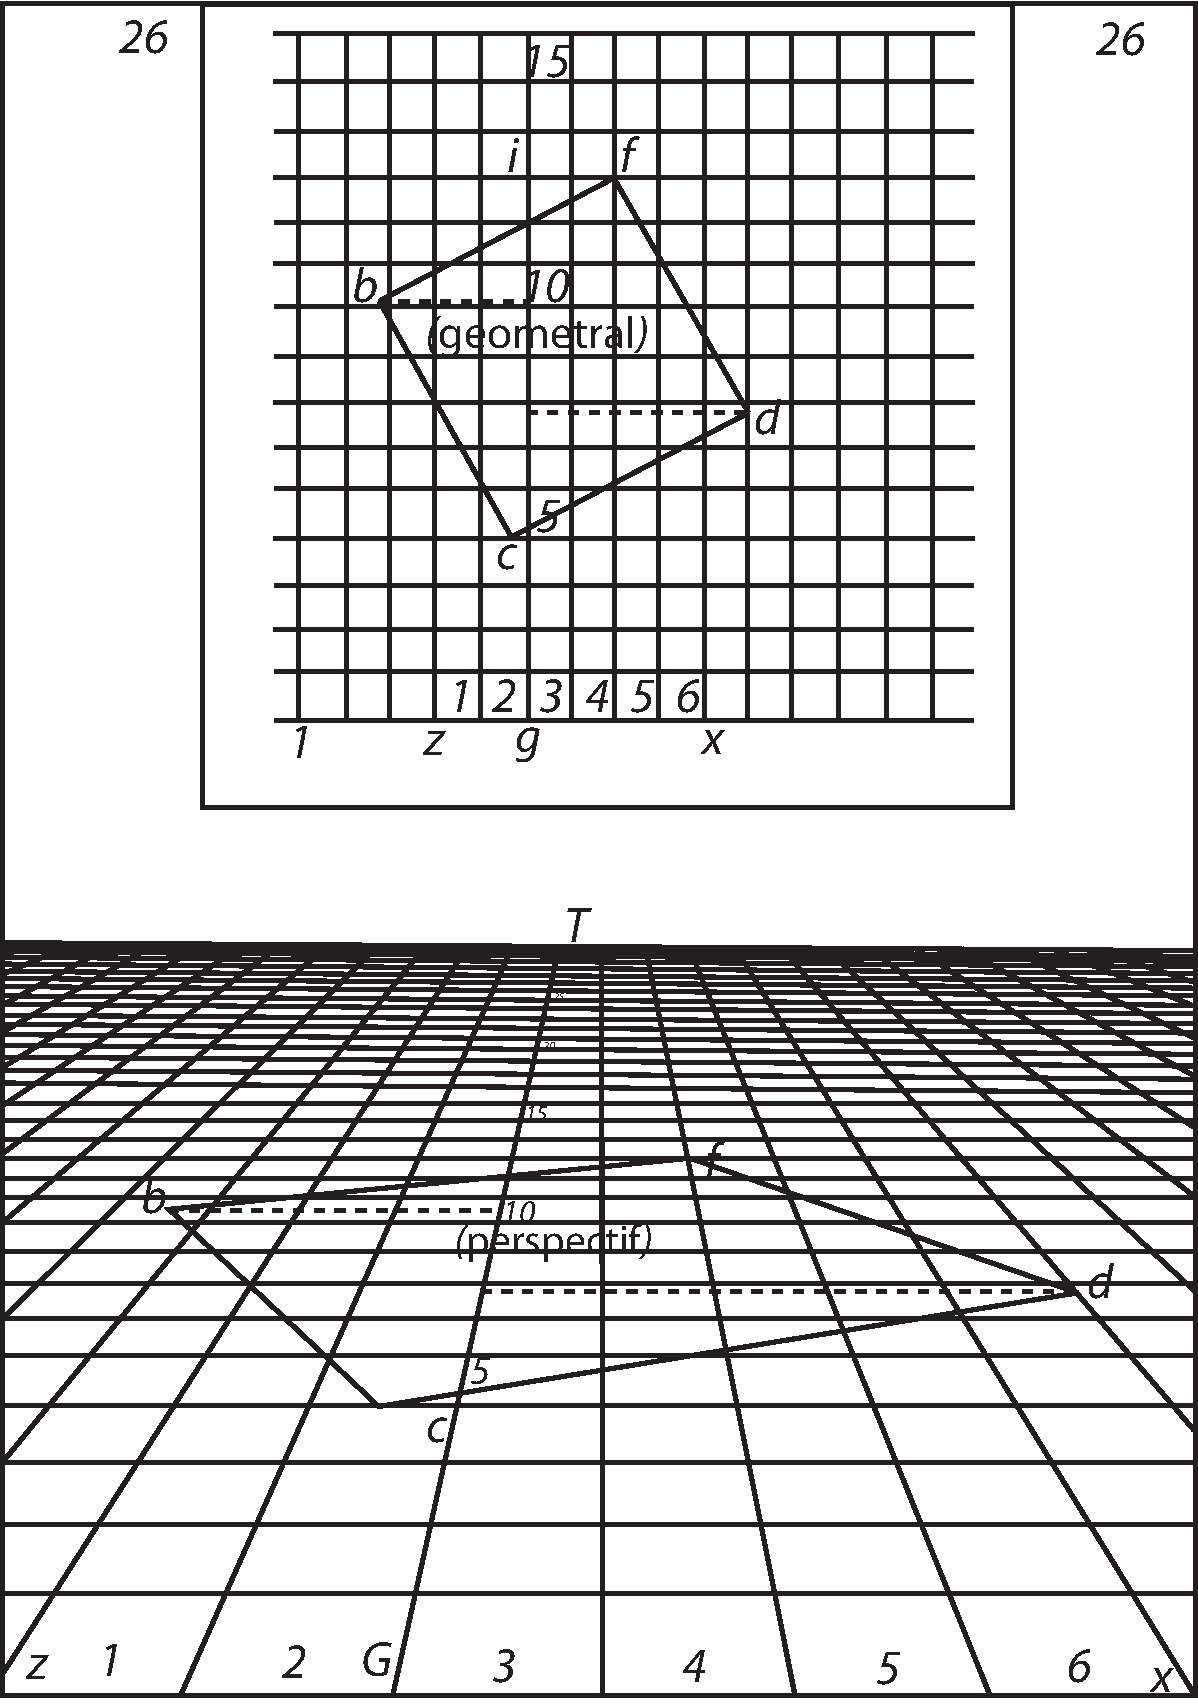
\includegraphics[width=0.8\textwidth]{images/T26-Desargues}
\\\rule[-4mm]{0mm}{10mm}\textit{[Fig. 10]}
\end{center}
\protect\clearpage
\pstart [p.~86] [...] en apres tirez au del\`{a} de cette conduite, \`{a} autant de ses pieds loin d'elle, que vous voulez que la hauteur de l'oeil\protect\index{Sachverzeichnis}{oeil} en contienne, vne droite ZCX, qui luy soit paralelle; elle sera celle qu'on nomme communement, \textit{horisontale}, et M. D.\footnote{\textit{Leibniz erg\"{a}nzt} M. D. \textit{zu} Mons. Desargues} ligne du plan de l'oeil\protect\index{Sachverzeichnis}{oeil}\footnote{\textit{Am Rand gestrichen}: la figure est fautive}; Dauantage, menez des deux bouts \textit{q} et \textit{p}, duquel que vous voudrez des pieds de la conduite de front E\textit{l}GV, comme icy par exemple de celuy \textit{4}, au point qu'il vous plaira C, de la ligne horisontale ZCX, deux droites fuyantes \textit{q}C, \textit{p}C; elles vous regleront entr'elles deux, l'inegalit\'{e} continuelle qu'il doit y auoir entre les pieds de front de c\'{e}t exemple; c'est \`{a} dire qu'elles en forment l'eschelle des pieds de front:\footnote{\textit{Leibniz unterstreicht}: l'eschelle [...] front} [...].\pend
\protect\clearpage
\begin{center}
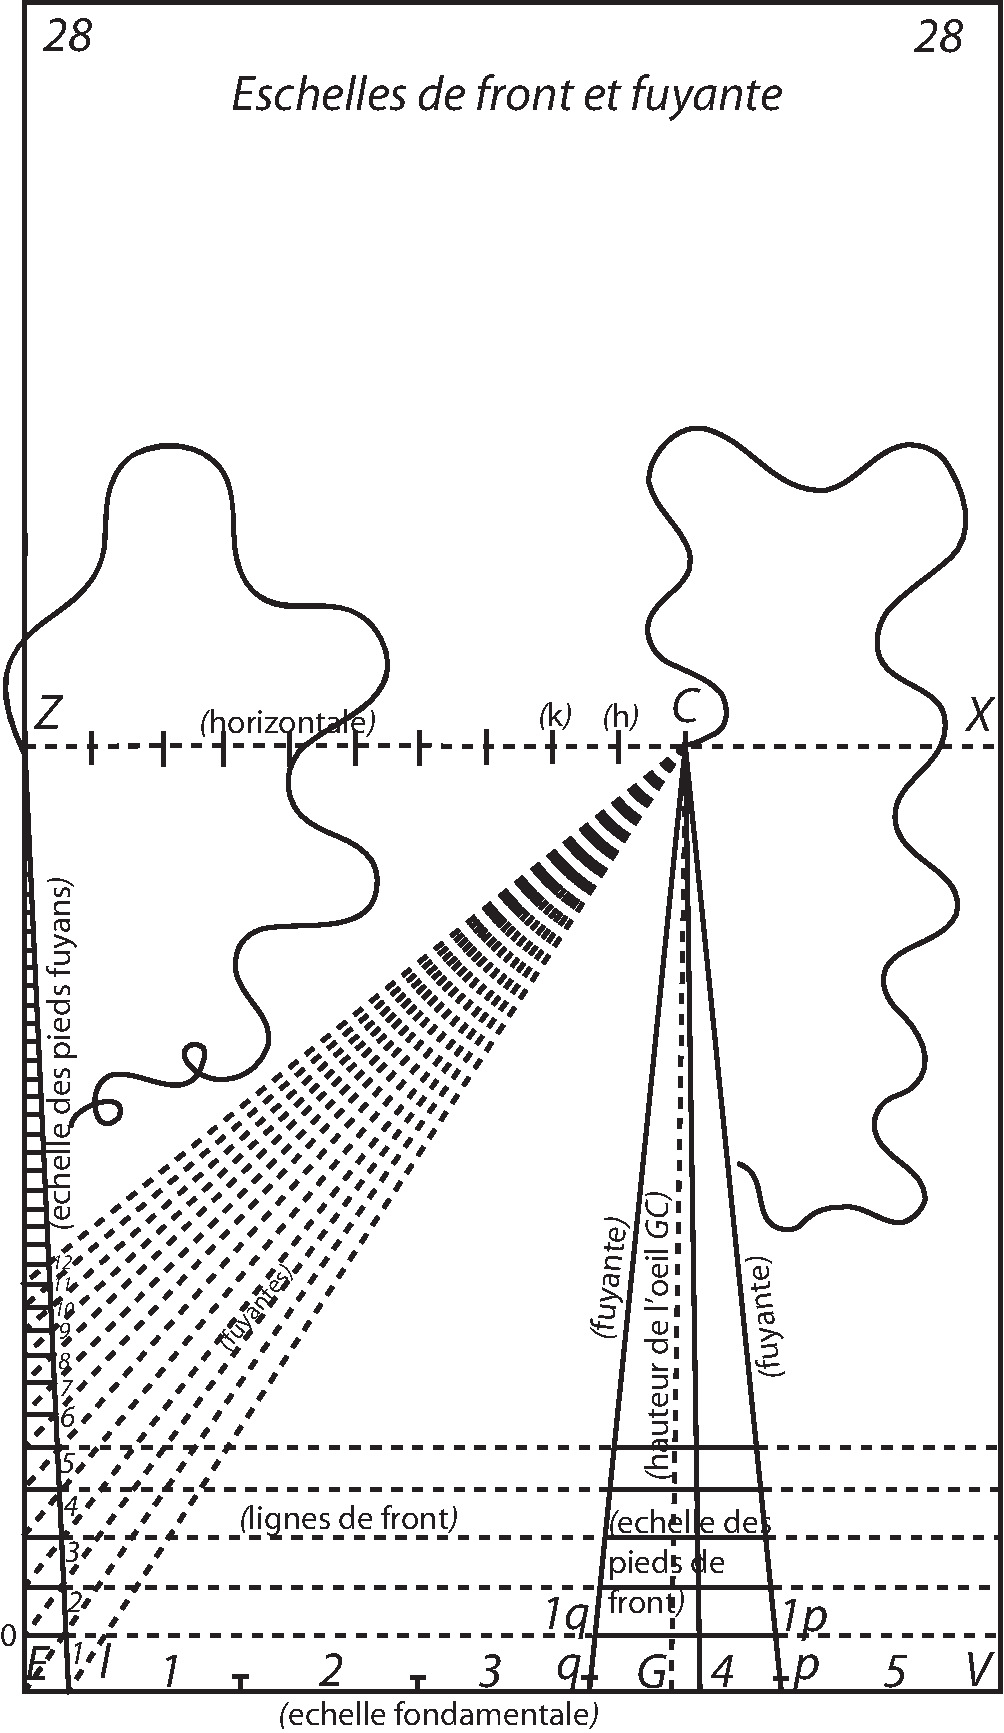
\includegraphics[width=0.6\textwidth]{images/T28-Desargues}
\\\rule[-4mm]{0mm}{10mm}\textit{[Fig. 11]}\textsuperscript{10}\\
\end{center}
\footnoterule
\pstart\noindent\textsuperscript{10}\textit{Unter der \"{U}berschrift}: \textso{Pieds de front} sont les parties des lignes de front; comprises entre deux fuyantes\protect\index{Sachverzeichnis}{echelle fuyante@\'{e}chelle!fuyante} men\'{e}es des deux bouts \textit{q}, \textit{p} d'un pied de l'echelle\protect\index{Sachverzeichnis}{echelle@\'{e}chelle}
\\
\footnoterule\\
fondamentale \textit{EV} \`{a} un point \textit{C} de la ligne horizontale; \textit{ZX}.\textso{ L'echelle}\protect\index{Sachverzeichnis}{echelle de front@\'{e}chelle!de front} de front est la suite des pieds de front compris entre deux m\^{e}mes fuyantes. Prenez dans l'echelle\protect\index{Sachverzeichnis}{echelle@\'{e}chelle} fondamentale, une droite \textit{EL}, qui est \`{a} un pied de l'echelle\protect\index{Sachverzeichnis}{echelle@\'{e}chelle} fondamentale \textit{qp} comme \textit{CZ} prise dans l'horizontale depuis le point \textit{C}, est \`{a} la distance de la station \`{a} la conduite de front. Men\'{e}s \textit{EZ}, \textit{lZ } les parties des lignes de front, comprises entre les deux fuyantes \textit{EZ}, \textit{lZ} seront les pieds fuyans et leur suite sera l'echelle\protect\index{Sachverzeichnis}{echelle@\'{e}chelle} des pieds fuyans.\\ \textit{In der Mitte unter der Geraden}: \textit{ZX}: \textit{ch}, \textit{hk}, etc. \'{e}gal \`{a} \textit{El}\\ \textit{Links unter der Geraden}: \textit{ZX}: \textit{CZ} est autant de fois \textit{El} que la distance de la station \`{a} la conduite de front, a des pieds de long.\\ \textit{Unter der Zeichnung links}: \textit{El}\textso{ pied fuyans fondamental.} \textit{NB}\\ \textit{Unter der Zeichnung}: Suppose \textit{ZE} parallele \`{a} \textit{CG} il se demontre que \textit{EO} est egale \`{a} \textit{1q1p} car \textit{EO} : \textit{ZO} :: \textit{El} : \textit{GE} :: \textit{qp} : \textit{CZ} :: \textit{1q1p} : \textit{ZO}. La figure est mal faite, car \textit{CZ} deuuroit estre \`{a} \textit{CG} comme \textit{El} \`{a} \textit{qp}, et les deux premiers estans faits quasi egaux. Les derniers le deuuroient estre \edtext{aussi. \selectlanguage{latin} }{\lemma{aussi}\Afootnote{\textbar\ supposant \textit{ZE} et \textit{CG} item \textit{CZ} et \textit{lE} paralleles et egales \textit{ gestr.}\ \textbar\ . \textit{L}}}\\ \textit{Unter der Zeichnung rechts}: \textso{pied de front fondamental} NB, et \textso{pied geometral} NB sont une m\^{e}me chose \textit{qp}.\\ \textit{Neben der Zeichnung rechts am Rand}: \textit{CG} hauteur de l'oeil \textit{qp} pied \edtext{geometral \textit{El}}{\lemma{geometral}\Afootnote{ \textbar\ egal si vous voul\'{e}s \`{a} \textit{pq} \textit{ gestr.}\ \textbar\ \textit{El}\ \textit{L}\hspace{6cm}}} pris \`{a} discretion\\
\protect\begin{tabular}{l}$CZ:CG::EL:qp$\\$EG\hspace{9pt}CZ$\protect\end{tabular}\\\textit{EO} : \textit{O1} :: \textit{EZ} : \textit{CZ} :: \textit{qp} : \textit{El}\textit{ZO} : \textit{O1} :: \textit{ZE} : \textit{El} \\\rule[-4mm]{0mm}{10mm} $\protect\overbrace{\frac{ZE\cdot EI}{qp}}^{E0\cdot CZ}\protect\overbrace{ZE - E0}^{\sqcap\hspace{5pt} Z0\hspace{5pt}EI}$ \\seu \textit{ZO} : \textit{EO} :: \textit{GE} : \textit{El}. Ergo $\displaystyle 1\sqcap\frac{CG}{E0} - \frac{CG}{qp}$ seu $\displaystyle E0\; \sqcap \frac{CG\cdot qp}{CG+qp}$ \\itaque \textit{EO} prodit eadem, qualiscunque sumatur \textit{El} $\displaystyle CZ \sqcap \frac{CG \cdot El}{qp}$.\rule[-4mm]{0mm}{10mm}\pend
\addtocounter{footnote}{1}
\protect\clearpage
\begin{center}
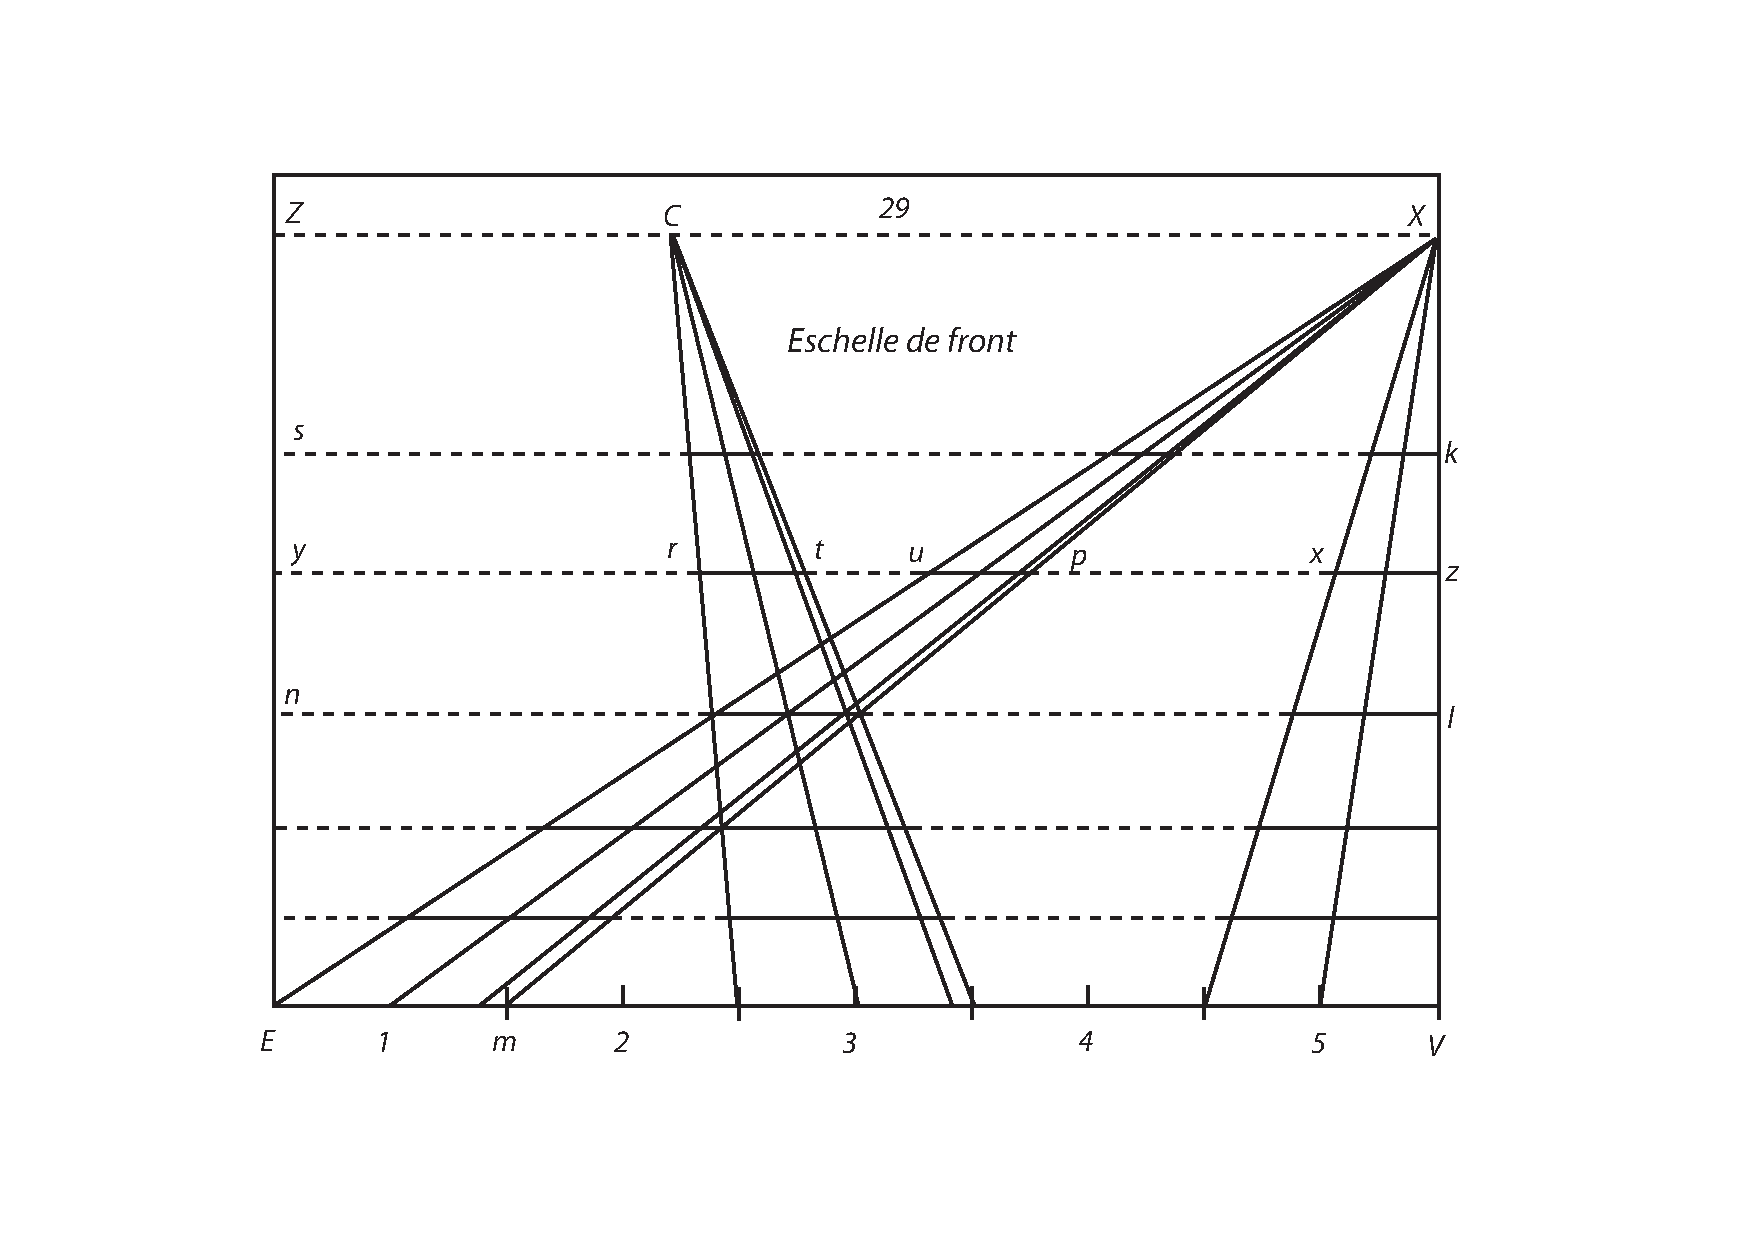
\includegraphics[width=1.0\textwidth]{images/T29-Desargues_87_a}\end{center}
\protect\rule[0cm]{6cm}{0cm}\textit{[Fig. 12a]}
\footnote{\textit{\"{U}ber der Strecke tu}: \textit{rt} \'{e}gal \`{a} \textit{up} ou \`{a} \textit{xz}}
\protect\clearpage
\begin{center}
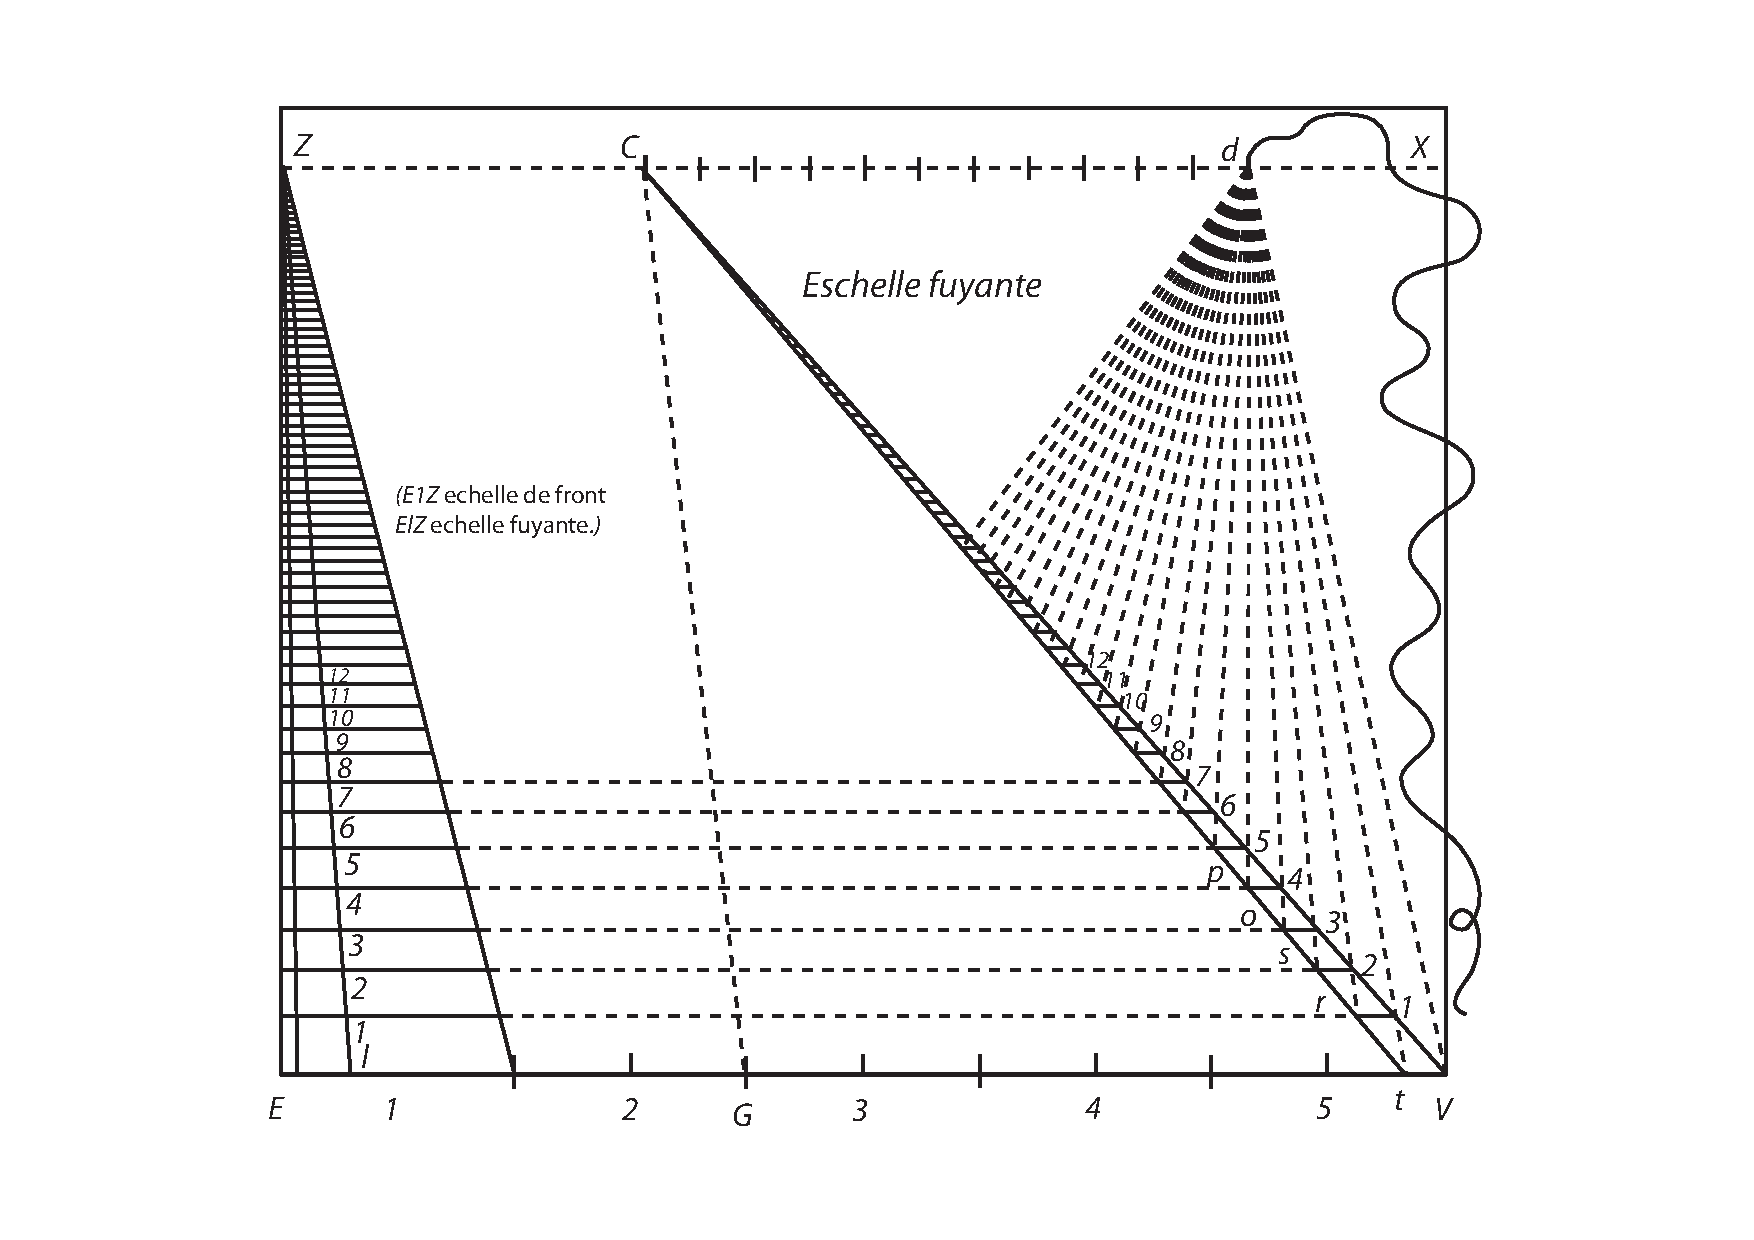
\includegraphics[width=0.95\textwidth]{images/T29-Desargues_87_b}
\\\textit{[Fig. 12b]}
\footnote{\textit{Links unter der Geraden ZX}: \textit{cd} \`{a} \textit{Vt} ou \`{a} \textit{dh} comme la distance de la station \`{a} la conduite de front est \`{a} un pied \textit{E1}. \\ \textit{Rechts unter der Geraden }\textit{ZX}: \textit{dh} \'{e}gal \`{a} \textit{Vt} \\ \textit{Oben links neben der Geraden CV}: \protect\begin{tabular}{c} dp\\do\protect\end{tabular} coupe \textit{CV} en \protect\begin{tabular}{c} 5\\4\protect\end{tabular}\rule[-4mm]{0mm}{10mm}  \\ \textit{Im unteren Teil der Abbildung in der Mitte links neben der Geraden CV}: \textit{E1Z} echelle de front\protect\index{Sachverzeichnis}{echelle de front@\'{e}chelle!de front} \textit{ElZ} echelle fuyante\protect\index{Sachverzeichnis}{echelle fuyante@\'{e}chelle!fuyante}.}
\end{center}